% numerical.tex

\cleardoublepage
\chapter{Optimised Ascent Trajectory}\label{chapter:Ascent}
	
%	\textcolor{red}{XXX NOTE third stage has very small thrust vector angle, turns out that the force is pretty close to the CG}
	
%	\textcolor{red}{XXX check all sig figs after all results are done, and see what they need to be, and reduce some if necessary}


	
This chapter presents a maximum payload-to-orbit trajectory optimisation for the representative launch system. 
This launch system is simulated as being launched from the Equatorial Launch Australia launch site in East Arnhem Land (Detailed in Section \ref{sec:mission}), and delivers a small satellite into sun synchronous orbit. LODESTAR is used to calculate the maximum payload-to-orbit trajectory solutions for this launch system.
First, a trajectory solution is calculated in which the scramjet accelerator flies at constant dynamic pressure. This trajectory is calculated to serve as a baseline for comparisons, as previous studies have assumed that flying the scramjet accelerator at its maximum allowable dynamic pressure would produce the best overall system performance\cite{Preller2017b}. An optimal payload-to-orbit trajectory is then developed, and the trajectory shape compared and contrasted to the constant dynamic pressure trajectory.
Lastly, a sensitivity study is performed, by varying key performance parameters of the launch system and investigating the effects of each parameter on the performance of the launch system. 

The following trajectories are developed: 
\begin{itemize}
	
	\item Case 1: $q = $ 50kPa fixed scramjet accelerator trajectory. \newline$\rightarrow$ This trajectory provides a baseline trajectory for comparison purposes.
	\item Case 2: Trajectory optimised for payload-to-orbit, $q_{max} = $ 50kPa. \newline$\rightarrow$ This trajectory demonstrates improved performance through trajectory optimisation.
	\item Case 3: Variation of maximum allowable dynamic pressure between $q_{max} = $ 45kPa \& $q_{max} = $ 55kPa. 
	\newline$\rightarrow$ Comparison of optimised trajectories allows the influence of the scramjet accelerator's ability to withstand aerodynamic forces on the launch system performance to be investigated.
	\item Case 4: Variation of the coefficient of drag of the scramjet accelerator between $C_d = 90\%$ \& $C_d = 110\%$. 
	\newline$\rightarrow$ Comparison of optimised trajectories allows the effects of the scramjet accelerator's aerodynamic design on the launch system performance to be investigated.
	\item Case 5: Variation of the specific impulse of the scramjet accelerator's C-REST engines between $I_{SP} = 90\%$ \& $I_{SP} = 110\%$. 
	\newline$\rightarrow$ Comparison of optimised trajectories allows the effects of the efficiency of the C-REST engines on the launch system performance to be investigated. 
	\item Case 6: Variation of the mass of the scramjet accelerator between $m_2 = 90\%$ \& $m_2 = 110\%$. 
	\newline$\rightarrow$ Comparison of optimised trajectories allows the effects of the internal design of the scramjet accelerator on the launch system performance to be investigated. 
	\item Case 7: Variation of the fuel mass of the scramjet accelerator between $m_{fuel} = 90\%$ \& $m_{fuel} = 110\%$. 
	\newline$\rightarrow$ Comparison of optimised trajectories allows the effects of the amount of fuel which the scramjet accelerator is able to carry on the launch system performance to be investigated. 
	\item Case 8: Variation of the mass of the third stage rocket between $m_3 = 90\%$ \& $m_3 = 110\%$. 
	\newline$\rightarrow$ Comparison of optimised trajectories allows the effects of the third stage internal design on the launch system performance to be investigated. 
	\item Case 9: Variation of the specific impulse of the third stage rocket between $I_{SP,3} = 90\%$ \& $I_{SP,3} = 110\%$. 
	\newline$\rightarrow$ Comparison of optimised trajectories allows the effects of the efficiency of the third stage engine on the launch system performance to be investigated. 
	\item Case 10: Variation of the coefficient of drag of the third stage rocket between $C_d = 90\%$ \& $C_d = 110\%$.
	\newline$\rightarrow$ Comparison of optimised trajectories allows the effects of the aerodynamic design of the third stage on the launch system performance to be investigated.
\end{itemize}
These optimised trajectory cases allow the benefits of flying an optimised trajectory to be quantified, and allow the impact of key design parameters on the performance of the launch system to be characterised. 

 \textcolor{red}{These optimised trajectories are presented in the following sections, along with key performance indicators and their sensitivities. These are presented to a number of significant figures judged necessary to adequately present the trajectory results and sensitivities to the accuracy of the trajectory simulation, with the caveat that the launch system modelling carries with it significant uncertainties.}
  

\section{Case 1: Constant Dynamic Pressure Trajectory}\label{sec:constq}

\begin{figure}[ht]% updated 15/8/19
	\centering
	\includegraphics[width=1\linewidth]{H:/github-home/LODESTAR-revisions/ArchivedResults/20190809T122214mode900/GroundTrackConstq}
	\caption{Maximum payload-to-orbit trajectory path with the scramjet accelerator flying at constant dynamic pressure (Case 1). Initial heading angle \textcolor{red}{91.4}$^\circ$.}
	\label{fig:GroundTrackConstq}
\end{figure}

The first trajectory that is produced using LODESTAR is a maximum payload-to-orbit trajectory in which the scramjet accelerator flies a constant dynamic pressure path, at its maximum allowable dynamic pressure of 50kPa. In order to drive the scramjet accelerator towards a constant dynamic pressure path, the cost function detailed in Table \ref{tab:SPARTANascentsetup} is utilised. In addition to the dynamic pressure cost function, the maximum payload-to-orbit cost function is also active on the third stage phase, so that once the scramjet accelerator flies close to 50kPa, the third stage will fly a maximum payload-to-orbit trajectory from the termination of the scramjet accelerator's constant dynamic pressure path.
Previous studies have assumed that flying the scramjet accelerator at constant dynamic pressure will produce the best possible system performance\cite{Preller2017b}. Because of this assumption, a constant dynamic pressure trajectory is produced to serve as a baseline for comparison with the maximum payload-to-orbit optimised trajectory. Producing a constant dynamic pressure trajectory also serves to verify that LODESTAR is able to calculate a trajectory in which the scramjet accelerator flies at a fixed dynamic pressure for the duration of its flight. 
In addition, the designs and aerodynamic simulations of each vehicle of the launch system have been improved in this work, compared to previous studies\cite{Preller2017b}. In this work, the internal design of the scramjet accelerator has been modified (as described in Section \ref{sec:SPARTAN}), the third stage design has been modified significantly (as described in Section \ref{sec:ThirdStageBaseline}), the first stage is included (as described in Section \ref{sec:firststage}), and Cart3D\cite{CART3D} is used for aerodynamic calculations (as detailed in Section \ref{sec:aero}). Simulating a constant dynamic pressure verifies that the first stage is able to reach the maximum dynamic pressure of the scramjet accelerator, and that the scramjet accelerator is able to fly at its maximum dynamic pressure within its control and aerodynamic limits. This verification ensures that any deviations from the scramjet accelerator's maximum dynamic pressure when flying a maximum payload-to-orbit trajectory serve to improve the performance of the system, rather than being a result of the problem setup or design constraints. 

\begin{table}[ht]% updated 14/8/19
	\centering
	
	\begin{tabular}{l c } 
		\hline \textbf{Trajectory Condition}
		&Value
		\\
		\hline \textbf{Payload to Orbit (kg)}
		& \textbf{\PayloadToOrbitConstqNoReturn}
		\\
		\textbf{Total $\eta_{exergy}$ (\%)}
		& \textbf{\totalExergyEffConstqNoReturn}
		\\
		\hline 
		\textbf{1$^{st}$ Stage $\eta_{exergy}$ (\%)}
		& \textbf{\firstExergyEffConstqNoReturn}
		\\
	
		\textbf{Separation Alt, 1$\rightarrow$2 (km)}
		& \firstsecondSeparationAltConstqNoReturn
		\\
		\textbf{Separation v, 1$\rightarrow$2 (m/s)}
		& \firstsecondSeparationvConstqNoReturn
		\\
		\textbf{Separation $\gamma$, 1$\rightarrow$2 (deg)}
		& \firstsecondSeparationgammaConstqNoReturn
		\\
		\hline 
		\textbf{2$^{nd}$ Stage $\eta_{exergy}$ (\%)}
		& \textbf{\secondExergyEffConstqNoReturn}
		\\
		\textbf{Separation Alt, 2$\rightarrow$3 (km)}
		& \secondthirdSeparationAltConstqNoReturn
		\\
		\textbf{Separation $v$, 2$\rightarrow$3 (m/s)}
		& \secondthirdSeparationvConstqNoReturn
		\\
		\textbf{Separation $\gamma$, 2$\rightarrow$3 (deg)}
		& \secondthirdSeparationgammaConstqNoReturn
		\\
		\textbf{2$^{nd}$ Stage Distance Flown (km)}
		& \SecondDistConstqNoReturn
		\\
		\hline 
		\textbf{3$^{rd}$ Stage $\eta_{exergy}$ (\%)}
		& \textbf{\thirddExergyEffConstqNoReturn}
		\\
	
		\textbf{3$^{rd}$ Stage $t$, $q >$ 5kpa (s)}
		& \thirdqOverFiveConstqNoReturn
		\\
		\textbf{3$^{rd}$ Stage Fuel Mass (kg)}
		& \thirdmFuelConstqNoReturn
		\\
		\hline 
	\end{tabular} 
	
	\caption{Summary of the key results from a maximum payload-to-orbit trajectory with the scramjet accelerator constrained to 50kPa (Case 1).}
	\label{tab:constqsummary} % updated 14/8/19
\end{table}
\begin{figure}[ht!] % updated 14/8/19
	\centering
	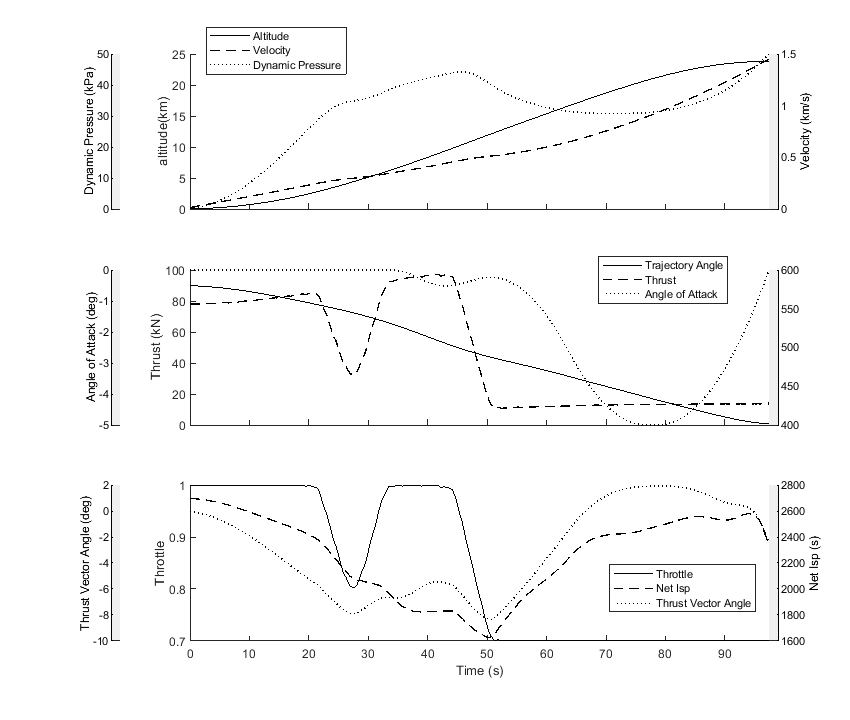
\includegraphics[width=0.9\linewidth]{H:/github-home/LODESTAR-revisions/ArchivedResults/20190809T122214mode900/FirstStageConstq}
	\caption{The first stage trajectory of the launch system, with the scramjet accelerator constrained to flight at constant dynamic pressure (Case 1).}
	\label{fig:FirstStageConstq}
\end{figure}
LODESTAR successfully computes the trajectory of the rocket-scramjet-rocket system, with the scramjet accelerator flying at constant dynamic pressure, achieving a payload-to-orbit of \PayloadToOrbitConstqNoReturn kg.
Figure \ref{fig:GroundTrackConstq} shows the optimised trajectory path, Figures \ref{fig:FirstStageConstq}-\ref{fig:ThirdStageConstq} show details of the optimised trajectory for each stage, and Table \ref{tab:constqsummary} provides a summary of the key parameters of the trajectory, including the exergy efficiency of each stage.
The rocket-scramjet-rocket system launches vertically, flying a fixed vertical trajectory for 3.9s, after which a pitchover is initiated. Under power of the first stage rocket, the launch system begins pitching, flying north-west, over the Arafura Sea. 
After pitchover the angle of attack stays constant at 0$^\circ$ for \textcolor{red}{99.9}s, as shown in Figure \ref{fig:FirstStageConstq}. At this point, the angle of attack is reduced, reaching a minimum of \textcolor{red}{-5.0}$^\circ$, before increasing back up to 0$^\circ$ for stage separation. \textcolor{red}{The first stage is throttled down temporarily at 20.3s flight time, to a minimum of 80.5\%. At 41.9s, the throttle is reduced to its minimum of 70\%, and maintained at this for the remainder of flight to assist in pitching. }
The scramjet accelerator is separated at a trajectory angle of \firstsecondSeparationgammaConstqNoReturn$^\circ$ at an altitude of \firstsecondSeparationAltConstqNoReturn km, at a flight time of \textcolor{red}{97.4}s, with a total ground distance of \FirstStageDistStandardNoReturn km covered under power of the first stage rocket. 
The first stage rocket achieves an exergy efficiency of \firstExergyEffConstqNoReturn\%$\eta$ when separating the scramjet accelerator onto a constant dynamic pressure trajectory. 


\begin{figure}[ht!]% updated 14/8/19
\centering
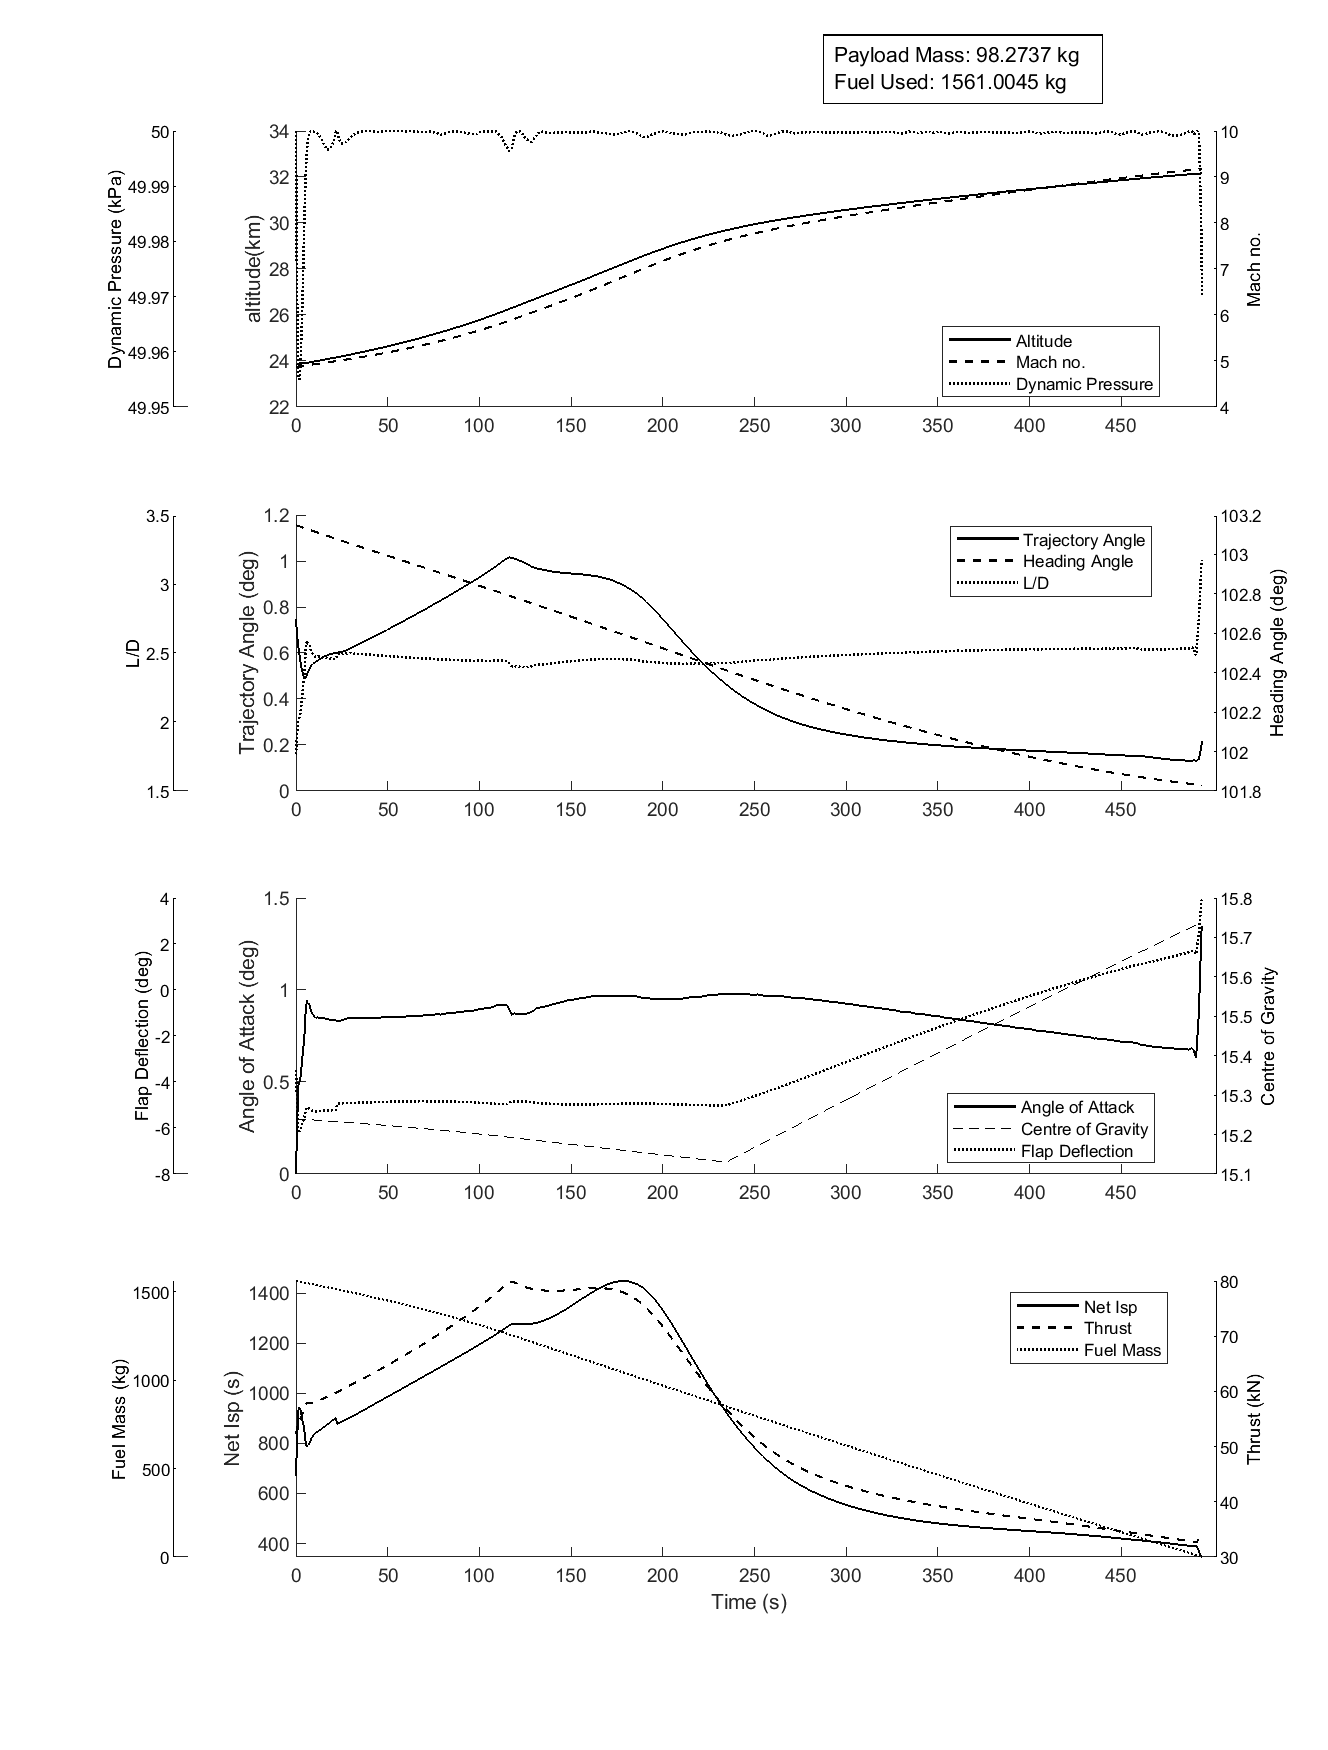
\includegraphics[width=0.9\linewidth]{H:/github-home/LODESTAR-revisions/ArchivedResults/20190809T122214mode900/SecondStageConstq}
\caption{The constant dynamic pressure flight path of the scramjet accelerator (Case 1).}
\label{fig:SecondStageConstq}
\end{figure}


The constant dynamic pressure trajectory for the scramjet accelerator stage is shown in Figure \ref{fig:SecondStageConstq}, with key results summarised in Table \ref{tab:constqsummary}. After the separation of the first stage rocket, the scramjet accelerator flies north west over the Arafura Sea, and crosses West Papua before releasing the third stage rocket. Due to the clear objective of a constant dynamic pressure trajectory, any deviations from the target dynamic pressure are readily apparent, allowing the efficacy of the optimiser to be verified. 
The constant dynamic pressure trajectory shows very close adherence to 50kPa dynamic pressure  throughout the trajectory (maximum 0.2\% deviation), indicating that scramjet accelerator flight at a constant dynamic pressure is able to be achieved.  
Over the trajectory, the Mach number increases from \textcolor{red}{4.88} to \textcolor{red}{9.18}, the speed increases from \firstsecondSeparationvConstqNoReturn m/s to \secondthirdSeparationvConstqNoReturn m/s, and the flap deflection increases from \textcolor{red}{-6.14}$^\circ$ to \textcolor{red}{a maximum of 3.93$^\circ$ during pull-up}. The angles of attack of the scramjet accelerator are low across the trajectory, generally between \textcolor{red}{0.6-1.0}$^\circ$, indicating that the lift of the scramjet accelerator is high for this mission profile. At the beginning of the trajectory the equivalence ratio increases, as the capture limitations are relaxed with increasing Mach number. This causes the net specific impulse ($I_{sp_{net}} = \frac{T-D}{\dot{m}_f g}$) to increase, to a maximum of \textcolor{red}{1448s}, during the first \textcolor{red}{180.4}s flight time.  After this initial increase, the net specific impulse decreases over the trajectory, as the efficiency of the scramjet engines decreases. 
Third stage release occurs at \textcolor{red}{591.4s flight time}, at \secondthirdSeparationAltConstqNoReturn km altitude. Immediately before third stage separation, there is a slight increase in the angle of attack and flap deflection of the scramjet accelerator. This is done to increase the trajectory angle and improve the payload-to-orbit slightly, but does not have a significant effect on the performance of the launch system. 

\begin{figure}[ht!]% updated 14/8/19
\centering
\includegraphics[width=0.9\linewidth]{H:/github-home/LODESTAR-revisions/ArchivedResults/20190809T122214mode900/ThirdStageConstq}
\caption{The third stage trajectory of the launch system, with the scramjet accelerator constrained to flight at constant dynamic pressure (Case 1).}
\label{fig:ThirdStageConstq}
\end{figure}

Figure \ref{fig:ThirdStageConstq} shows the corresponding third stage atmospheric exit trajectory after release, evaluated as described in Chapter \ref{chapter:LODESTAR}. The \textcolor{red}{flight path of the} third stage released from a constant dynamic pressure trajectory, shown in Figure \ref{fig:ThirdStageConstq}, stays close to horizontal for the first \textcolor{red}{12}s of flight. This slow ascent leads to the rocket spending a large amount of time at low altitude, in a high drag environment, spending \thirdqOverFiveConstqNoReturn s at over 5kPa dynamic pressure. The angle of attack increases gradually to a maximum of \textcolor{red}{10}$^\circ$ at \textcolor{red}{27.8}s \textcolor{red}{and is then maintained at the maximum 10$^\circ$ until 111.7s, when the angle of attack is reduced slightly, increased to the maximum briefly, and finally reduced to 0$^\circ$ for burnout at 146.2s}. The dynamic pressure of the third stage rocket reduces to 10kPa at \textcolor{red}{188.2}s, at which point the heat shield is discarded. The rocket coasts to a trajectory angle of 0$^\circ$, which is reached at a total flight time of \textcolor{red}{827.6}s. The trajectory terminates at 90km, the lowest allowable altitude for circularisation. 
When this altitude is reached, the trajectory is circularised and a Hohmann transfer manoeuvre is performed to reach sun synchronous orbit.






\section{Case 2: Optimised Ascent Trajectory}\label{sec:optimisednoreturn}

This section presents the maximum payload-to-orbit trajectory for the rocket-scramjet-rocket launch system, with the scramjet accelerator able to deviate from its maximum dynamic pressure. 
The optimal trajectory shape for a 50kPa dynamic pressure limited trajectory is shown in Figure \ref{fig:GroundTrackStandardNoReturn}, with detailed trajectory information for each stage shown in Figures \ref{fig:FirstStageStandardNoReturn} - \ref{fig:ThirdStageStandardNoReturn}, and key results summarised in Table \ref{tab:summaryStandardNoReturn}. The maximum payload-to-orbit trajectory shape involves the scramjet accelerator performing altitude raising manoeuvres, where the dynamic pressure of the scramjet accelerator is lowered from its maximum of 50kPa. These manoeuvres serve either to increase the net specific impulse of the scramjet accelerator, or to trade-off the efficiency of the scramjet accelerator in order to increase the efficiency of the first and third stages. 
This payload-to-orbit optimised trajectory is able to deliver \PayloadToOrbitStandardNoReturn kg of payload to heliocentric orbit, an increase of \textcolor{red}{59.1}\% over the constant, 50kPa dynamic pressure result (Case 1).

\begin{figure}[ht!]%updated 15/8/19
	
	
	
	\centering
	\includegraphics[width=1\linewidth]{H:/github-home/LODESTAR-revisions/ArchivedResults/20190723T125843mode10/GroundTrackStandard}
	\caption{The optimised maximum payload-to-orbit trajectory of the launch system (Case 2).}
	\label{fig:GroundTrackStandardNoReturn}
\end{figure}


The first stage, shown in Figure \ref{fig:FirstStageStandardNoReturn}, \textcolor{red}{flies a different} trajectory to that of the first stage releasing the scramjet accelerator onto a constant dynamic pressure trajectory.
\begin{figure}[ht!]% updated 14/8/19
	\centering
	\includegraphics[width=0.9\linewidth]{H:/github-home/LODESTAR-revisions/ArchivedResults/20190723T125843mode10/FirstStageStandard}
	\caption{The optimised maximum payload-to-orbit trajectory of the launch system under power of the first stage rocket (Case 2).}
	\label{fig:FirstStageStandardNoReturn}
\end{figure}
 The trajectory angle at the separation of the scramjet accelerator is \secondthirdSeparationgammaqStandardNoReturn$^\circ$, rather than the trajectory angle of \secondthirdSeparationgammaConstqNoReturn$^\circ$ required for the scramjet accelerator to fly a constant dynamic pressure trajectory. Additionally, the altitude at first-second stage separation is raised to \firstsecondSeparationAltStandardNoReturn km, an increase of \textcolor{red}{0.68}km compared to the separation point of a scramjet accelerator flying at constant 50kPa dynamic pressure. This higher release angle and altitude causes the altitude of the scramjet accelerator to initially increase, and consequently for its dynamic pressure to decrease. This increased trajectory angle at separation is the consequence of a trade-off between the efficiency of the scramjet accelerator and the efficiency of the first stage. \textcolor{red}{In particular, while the first stage is still throttled down twice, at 19.7s and 62.7s, it is throttled down for much less total time than the first stage separating onto a constant dynamic pressure trajectory. }
 The efficiency of the first stage is increased to \firstExergyEffStandardNoReturn\%$\eta$ due to the increased acceleration \textcolor{red}{that this reduced throttling affords}, an overall improvement of \textcolor{red}{+0.623\%$\eta$ (+9.96\%)} compared to the first stage separating the scramjet accelerator at 50kPa conditions. 
 During the maximum payload-to-orbit trajectory, the first stage rocket releases the scramjet accelerator at a speed of \firstsecondSeparationvStandardNoReturn m/s, an increase of \textcolor{red}{5.7}\% compared to the first stage releasing the scramjet accelerator onto a constant dynamic pressure trajectory.


\begin{table}[ht]% updated 14/8/19
	\centering
\begin{tabular}{l c } 
	\hline \textbf{Trajectory Condition}
	& Value
	\\
	\hline \textbf{Payload to Orbit (kg)}
	& \textbf{\PayloadToOrbitStandardNoReturn}
	\\
	& \small(-147.6, +82.4)
	\\
	\textbf{Total $\eta_{exergy}$ (\%)}
	& \textbf{\totalExergyEffStandardNoReturn}
	\\
	\hline 
	\textbf{1$^{st}$ Stage $\eta_{exergy}$ (\%)}
	& \textbf{\firstExergyEffStandardNoReturn}
	\\

	\textbf{Separation Alt, 1$\rightarrow$2 (km)}
	& \firstsecondSeparationAltStandardNoReturn
	\\
	\textbf{Separation v, 1$\rightarrow$2 (m/s)}
	& \firstsecondSeparationvStandardNoReturn
	\\
	\textbf{Separation $\gamma$, 1$\rightarrow$2 (deg)}
	& \firstsecondSeparationgammaStandardNoReturn
	\\
	\hline 
	\textbf{2$^{nd}$ Stage $\eta_{exergy}$ (\%)}
	& \textbf{\secondExergyEffStandardNoReturn}
	\\

	\textbf{Separation Alt, 2$\rightarrow$3 (km)}
	& \secondthirdSeparationAltStandardNoReturn
	\\
	\textbf{Separation $v$, 2$\rightarrow$3 (m/s)}
	& \secondthirdSeparationvStandardNoReturn
	\\
	\textbf{Separation $\gamma$, 2$\rightarrow$3 (deg)}
	& \secondthirdSeparationgammaStandardNoReturn
	\\
	\textbf{2$^{nd}$ Stage Distance Flown (km)}
	& \SecondDistStandardNoReturn
	\\
	\hline 
	\textbf{3$^{rd}$ Stage $\eta_{exergy}$ (\%)}
	& \textbf{\thirddExergyEffStandardNoReturn}
	\\

	\textbf{3$^{rd}$ Stage $t$, $q >$ 5kpa (s)}
	& \thirdqOverFiveStandardNoReturn
	\\
	\textbf{3$^{rd}$ Stage Fuel Mass (kg)}
	& \thirdmFuelStandardNoReturn
	\\
	\hline 
\end{tabular} 
	\caption{A summary of key results from the maximum payload-to-orbit trajectory (Case 2).}
	\label{tab:summaryStandardNoReturn}
\end{table}







\begin{figure}[ht!]% updated 14/8/19
\centering
\includegraphics[width=0.9\linewidth]{H:/github-home/LODESTAR-revisions/ArchivedResults/20190723T125843mode10/SecondStageStandard}
\caption{The optimised maximum payload-to-orbit trajectory of the scramjet accelerator (Case 2).}
\label{fig:SecondStageStandardNoReturn}
\end{figure}



After the initial deviation from the maximum dynamic pressure, the scramjet accelerator returns to 50kPa dynamic pressure for a time. 
At \textcolor{red}{184.9} seconds flight time, the altitude of the trajectory is again raised, and the dynamic pressure decreased, to a minimum of \textcolor{red}{43.0}kPa. In this region the net specific impulse of the scramjet accelerator is relatively homogeneous with respect to changes in dynamic pressure, as can be observed in the specific impulse of the C-REST engines in Figure \ref{fig:IspStandard}. The homogeneity between flight conditions means that the variation in engine performance with flight conditions is small and that flying at the maximum dynamic pressure in this region does not maximise the specific impulse from the C-REST engines. Figure \ref{fig:NetIspStandardNoReturn} shows that while the optimised trajectory differs significantly from a constant dynamic pressure trajectory, both achieve similar net specific impulses during the acceleration phase of flight, with the exception of the initial trajectory conditions at Mach 5, where the efficiency of the scramjet accelerator is traded for first stage rocket performance. 
Appendix \ref{sec:Appendix_qconst} details a maximum payload-to-orbit trajectory in which the scramjet accelerator is constrained to 50kPa between Mach 6-8, to prevent the altitude raising manoeuvre from taking place. This constrained trajectory allows for the magnitude of the performance gain from the altitude raising manoeuvre to be quantified. 
Overall, the altitude raising manoeuvre results in a slight increase in net specific impulse, compared to the trajectory constrained to maximum $q$, increasing the overall efficiency of the launch system from \totalExergyEffqconstrainedNoReturn \%$\eta$ to \totalExergyEffStandardNoReturn\%$\eta$. This is a relatively minor variation, and the payload-to-orbit benefits of this altitude raising manoeuvre are correspondingly small; 
the optimised trajectory exhibits a payload-to-orbit increase of 0.5kg compared to the trajectory constrained to 50kPa between Mach 6-8, a difference of only 0.3\%.
However, it is important to note that, while its benefits are small, the altitude raising manoeuvre is consistently observed in all maximum payload-to-orbit optimised trajectories in which dynamic pressure is unconstrained, and this manoeuvre is similar to the manoeuvres observed by Fujikawa et al.\cite{Fujikawa2017} is their study of the Jaxa TSTO Spaceplane, though to a much lesser extent. 
Also, despite its small benefit to payload-to-orbit, this altitude raising manoeuvre is significant as it reduces the heating and structural loading on the scramjet accelerator. 





\begin{figure}[ht!]% updated 14/8/19 - note, modified point location for Mach 8.5 so not to be during pull-up
	\centering
	\includegraphics[width=\linewidth]{H:/github-home/LODESTAR-revisions/ArchivedResults/20190723T125843mode10/NetIspStandard}
	\caption{Net Isp contours for the scramjet accelerator at Mach numbers from 5-9, showing flight conditions for an optimised trajectory with no constraints (Case 2) and a constant dynamic pressure trajectory (Case 1). }
	\label{fig:NetIspStandardNoReturn}
\end{figure}

\begin{figure}[ht!]% updated 14/8/19 
	\centering
	\includegraphics[width=0.8\linewidth]{H:/github-home/LODESTAR-revisions/ArchivedResults/20190723T125843mode10/IspStandard}
	\caption{The specific impulse of the C-REST engines, plotted for inlet temperature (T1) and inlet Mach number (M1). Data points are shown in black.}
	\label{fig:IspStandard}
\end{figure}


At \textcolor{red}{319.4}s, the scramjet accelerator returns to flight at close to 50kPa dynamic pressure until \textcolor{red}{511.1}s. \textcolor{red}{During this time, a series of four small manoeuvres are performed, increasing the angle of attack of the scramjet accelerator briefly, and then reducing it in succession. These manoeuvres allow for longer periods of flight at lower angles of attack, where the net specific impulse of the scramjet accelerator is improved. }
 
 At 511.1s a pull-up manoeuvre is performed, gaining altitude until the third stage rocket is released at \textcolor{red}{543.7}s of scramjet accelerator flight time. 
 The point at which the pull-up manoeuvre begins is the location that takes into account the best combination of speed, altitude and release angle for the trade-off between the scramjet stage performance and the release of the third stage rocket. This pull-up indicates the region at which increasing altitude and release angle becomes more important than extracting maximum thrust from the scramjet (which is generally attained at high $q$ and low flight angle at an equivalence ratio of 1).
At high Mach numbers, flight in a lower dynamic pressure environment results in less thrust output from the scramjet engines, as well as an increase in angle of attack and flap deflection angle to compensate for the additional lift required. Due to this, less overall acceleration is obtained compared to the fixed dynamic pressure result. Separation occurs at a speed of \secondthirdSeparationvStandardNoReturn m/s, a decrease of \textcolor{red}{145.0}m/s (\textcolor{red}{-5.2}\%). However, at the same time separation altitude increases by \textcolor{red}{11.65}km (+\textcolor{red}{36.2}\%) to \secondthirdSeparationAltqStandardNoReturn km, resulting in a decrease in separation dynamic pressure to \secondthirdSeparationqStandardNoReturn kPa. 
\begin{figure}[ht!]% updated 14/8/19
	\centering
	\includegraphics[width=0.9\linewidth]{H:/github-home/LODESTAR-revisions/ArchivedResults/20190723T125843mode10/ThirdStageStandard}
	\caption{The third stage trajectory of the launch system flying the maximum payload-to-orbit trajectory (Case 2).}
	\label{fig:ThirdStageStandardNoReturn}
\end{figure}
The scramjet stage pull-up assists the rocket in manoeuvring to exoatmospheric altitude by increasing the altitude and angle at separation, utilising the superior aerodynamics and manoeuvrability of the scramjet accelerator. The increase in release angle, to the optimal angle of \secondthirdSeparationgammaStandardNoReturn$^\circ$, significantly reduces the turning that is required by the rocket as evident from comparing Fig \ref{fig:ThirdStageConstq} and \ref{fig:ThirdStageStandardNoReturn}. 
Overall, the altitude raising manoeuvres that the scramjet accelerator performs result in a decrease in the exergy efficiency of the scramjet accelerator to \secondExergyEffStandardNoReturn\%$\eta$, a total decrease of \textcolor{red}{-0.719}\%$\eta$ (-\textcolor{red}{14.04}\%) compared to the scramjet accelerator flying at a constant dynamic pressure. However, the optimised trajectory drastically increases the exergy efficiency of the third stage, to \thirddExergyEffStandardNoReturn\%$\eta$, an overall increase of +\textcolor{red}{6.013}\%$\eta$ (\textcolor{red}{+63.20}\%) compared to the third stage released from the scramjet accelerator flying a fixed dynamic pressure trajectory.  
Along with the increased efficiency of the first stage, this exergy trade-off leads to the total exergy efficiency of the launch system increasing, from \totalExergyEffConstqNoReturn\%$\eta$ to \totalExergyEffStandardNoReturn\%$\eta$. 

\textcolor{red}{
 This pull-up under airbreathing power is somewhat similar to the pull-ups that were observed in some of the previous studies of multi-stage airbreathing launch systems in Section \ref{sec:twostagelaunchers}, namely the LaRC Turboramjet\cite{Wilhite1991}, the JAXA TSTO Spaceplane\cite{Fujikawa2017}, and the XCALIBUR\cite{Bradford2002}. However, all of these pull-ups were either performed specifically to lower dynamic pressure for the orbiter stage\cite{Wilhite1991,Bradford2002}, or to improve the operation of the airbreathing engines\cite{Fujikawa2017}. The pull-up in this study is shown to directly improve the efficiency of the launch system, without improving the performance of the scramjet engines. This indicates that in addition to separation conditions that are beneficial for the design of the orbiter identified in these previous studies, the pull-up at the end of the airbreathing trajectory can directly improve the payload-to-orbit performance of the launch system. }

The trajectory of the third stage rocket after release from an optimised scramjet trajectory is shown in Figure \ref{fig:ThirdStageStandardNoReturn}. Release at a higher, more optimal angle, reduces the aerodynamic moment necessary to trim the vehicle. In turn, this reduced moment reduces the necessary thrust vector angle significantly. The third stage rocket is released at a high trajectory angle, and continuously gains altitude, avoiding the close-to-horizontal flight required by the fixed dynamic pressure release (Case 1).
Due to the higher altitude and release angle, the third stage rocket is released at a lower dynamic pressure, \secondthirdSeparationqCdStandardNoReturn kPa compared to \secondthirdSeparationqConstqNoReturn kPa, and spends much less time flying in a high dynamic pressure environment, \thirdqOverFiveStandard s at over 5kPa dynamic pressure rather than \thirdqOverFiveConstqNoReturn s. 
The reduced time that the rocket must spend in a high dynamic pressure environment, and the decrease in the maximum dynamic pressure that the rocket stage experiences, may allow the structural mass and heat shielding necessary to achieve exoatmospheric flight to be decreased, and may enable higher payload to orbit. \textcolor{red}{This possible improvement in payload-to-orbit is explored further in Appendix \ref{sec:TPSredesign}. In addition to improved payload-to-orbit, releasing the rocket at lower dynamic pressure reduces the thrust vector angle significantly, to below 1$^\circ$, compared to the angles of close to 7$^\circ$ reached during ascent after release from a scramjet accelerator flying at constant dynamic pressure. These reduced thrust vector angles would likely improve the controllability of the third stage rocket considerably, although detailed investigation of the controllability of the third stage rocket is beyond the scope of this study.} 


\textcolor{red}{
	\section{Discussion of Uncertainties}\label{sec:unc}
}


The aerodynamic and propulsive properties of the launch system that have been presented in this section are modelled using medium and low fidelity methods essential to allow full system trajectory optimisation to be carried out efficiently. These methods bring with them an associated uncertainty in the values that are calculated for the aerodynamic and propulsive performance of a vehicle, including those presented in Sections \ref{sec:propulsion}-\ref{sec:trimmedongineoff}, \ref{sec:firststageaero}, and \ref{sec:thirdstageprop}-\ref{sec:thirdstageaero}. These uncertainties are estimated in Appendix \ref{sec:aerounc} from previous studies that have compared the medium-to-low fidelity tools used to analyse propulsion and aerodynamics with high fidelity tools and experimental results. Previous error magnitudes are used to estimate the error magnitudes in the current study, with the maximum applicable error magnitude being used. The final values obtained from this study are replicated in Table \ref{tab:AppendixUncertaintyCopy}. The presence of these uncertainties may mean that the performance of the vehicle is significantly different to expected, producing significantly different payloads-to-orbit to those calculated. 

\begin{table}[ht]
	\centering
	\begin{tabular}{|c|c|c|c|}
		\hline  Uncertainty & Subsonic & Transonic  & Supersonic/Hypersonic \\ 
		\hline  1$^{st}$ \& 3$^{rd}$ Stage $I_{SP}$ & 1.3\% & 1.3\% &  1.3\% \\ 
		\hline  Scramjet $I_{SP}$ & - & - &  25\% \\ 
		\hline   $C_L$ & 17\% & 28.7\% & 12\% \\  
		\hline   $C_D$ & 33\% & 21\% & 11\% \\  
		\hline   $C_M$  & 23\% & 67.1\% &  22.0\% \\ 
		\hline 
	\end{tabular}
	\caption{The uncertainty margins associated with the aerodynamic and propulsive modelling, determined in Appendix \ref{tab:AppendixUncertaintyCopy}.}
	\label{tab:AppendixUncertaintyCopy}
\end{table}


A Monte-Carlo study is conducted in using these uncertainty bounds, with further details available in Appendix \ref{sec:uncquant}. The parameters in \ref{tab:AppendixUncertaintyCopy} are independently varied according to a Latin Hypercube analysis method to create a series of distinct cases, with each parameter in each regime multiplied by a constant within the uncertainty range, and maximum payload-to-orbit trajectories developed for each perturbed case. 
Analysis using the percentile method yields a 97.5\% confidence interval of 8.8-238.8kg in payload-to-orbit due to aerodynamic and propulsion modelling uncertainties, illustrating the large uncertainties still present in the modelling of airbreathing launch systems that are to be expected when using low-to-medium fidelity tools, as is the norm in the conceptual design phases, particularly given the general sensitivity of the payload mass in launch systems to variations in the launch system performance. However, this interval also indicates that producing a positive payload-to-orbit is likely to be possible under the current modelling scheme, although it is evident that more detailed analysis of this system is necessary before an accurate payload-to-orbit value is able to be attained. This said, the payload-to-orbit values calculated in this study are only intended as an indication of the performance possible using this launch system. The primary usefulness of these trajectories is in the studies of the optimal trajectory shape and performance trade-offs, and the comparison studies of the trends in performance that have been analysed in Chapters \ref{sec:sensitivityNoReturn} and \ref{sec:sensitivity}. 
%-XXX change this to no-return uncertainty

\section{Energy Usage Analysis}\label{sec:exergy1}

%\textcolor{red}{XXX  it might be better to describe propulsion inefficiencies as availability losses, or irreversibility. see https://ntrs.nasa.gov/archive/nasa/casi.ntrs.nasa.gov/20150009419.pdf,  need to look at Exergy Analysis
%	and Design Optimization for Aerospace Vehicles and
%	Systems} - I think for my application propulsion inefficicneies is an ok term


% From wikipedia: Specific impulse is often used as the unit of efficiency for rockets, since in the case of the rocket, there is a direct relation between specific impulse, specific fuel consumption and exhaust velocity. This direct relation is not generally present for airbreathing engines, and so specific impulse is less used in the literature. 
% hard to directly compare... and Isp is not directly efficiency. Also scramjet is obtaining energy from air. 

% These lowered propulsion losses are due to the scramjet accelerator's engines utilising atmospheric oxygen as an oxidiser, resulting in a higher propulsion system efficiency.
% I think this is wrong, airbreathing doesnt allow better FUEL uilisation necessarily, but doesnt need to store oxidiser.

% Remember higher IsP is lower efficiency for rockets

% 
%https://web.stanford.edu/~cantwell/AA103_Course_Material/RocketPerformanceNotes_J_Dyer.pdf
% https://ntrs.nasa.gov/archive/nasa/casi.ntrs.nasa.gov/20150009419.pdf

% think of a 'hovering' case, where all ther losses wuld be availability and propulsion losses, all energy just going into exhaust rater than rocket. This makes sense for the trends in the third stage. 

% remember to think of efficiency as instantaneous.

% Most of the work done by a rocket early in flight is "invested" in the kinetic energy of the propellant not yet burned, part of which they will release later when they are burned. 

% oberth effect for interest

\begin{table}[ht] % updated 29/12/19, note, ive just rounded the numbers, even though they dont quite add up right, seems most logical
	\centering
	\begin{tabular}{l c c} 
		\hline \textbf{Trajectory Condition}
		&50kpa Constant $q$
		&No $q$ Constraint
		\\
		\textbf{First Stage Fuel Exergy} 
		&\textbf{\firstEnergyConstqNoReturn} GJ
		&\textbf{\firstEnergyStandardNoReturn} GJ
		\\
		
		\textcolor{blue}{KE + PE of Payload}
		& \firstWpayloadConstqNoReturn \% (0.13 GJ)
		& \firstWpayloadStandardNoReturn \% (0.22 GJ)
		\\
		\textcolor{red}{KE + PE of  2$^{nd}$ \& 3$^{rd}$ Stage}
		& \firstWnextStageConstqNoReturn \% (12.50 GJ) & \firstWnextStageStandardNoReturn \% (13.66 GJ)
		\\
		
		\textcolor{red}{Overcoming Drag} 
		& \WDoneConstqNoReturn \% (5.57 GJ) & \WDoneStandardNoReturn \% (5.03 GJ)
		\\
		\textcolor{red}{KE + PE of 1$^{st}$ Stage Structural Mass} 
		& \WoneConstqNoReturn \% (1.86 GJ) & \WoneStandardNoReturn \% (2.04 GJ)
		\\ 
		\textcolor{red}{KE + PE of 1$^{st}$ Stage Fuel Mass} 
		& \WmFoneConstqNoReturn \% (5.00 GJ) & \WmFoneStandardNoReturn \% (5.39 GJ)
		\\ 
		\textcolor{red}{Propulsion Inefficiency} 
		& \PlossoneConstqNoReturn \% (176.83 GJ) & \PlossoneStandardNoReturn \% (175.56 GJ)
		\\ 
		\textbf{Scramjet Accelerator Fuel Exergy} 
		& \textbf{\secondEnergyConstqNoReturn} GJ & \textbf{\secondEnergyStandardNoReturn} GJ
		\\
		\textcolor{blue}{KE + PE of Payload}
		& \secondWpayloadConstqNoReturn \% (0.28 GJ) & \secondWpayloadStandardNoReturn \% (0.39 GJ) 
		\\
		\textcolor{red}{KE + PE of 3$^{rd}$ Stage}
		& \secondWnextStageConstqNoReturn \% (9.31 GJ) & \secondWnextStageStandardNoReturn \% (7.85 GJ)
		\\
		\textcolor{red}{Overcoming Drag}
		& \WDsecondConstqNoReturn \% (35.00 GJ) & \WDsecondStandardNoReturn \% (38.08 GJ)
		\\
		\textcolor{red}{KE + PE of scramjet accelerator Structural Mass}  
		& \WsecondConstqNoReturn \% (14.41 GJ) & \WsecondStandardNoReturn \% (12.39 GJ)
		\\
		\textcolor{red}{KE + PE of scramjet accelerator Fuel Mass}  
		& \WmFsecondConstqNoReturn \% (2.49 GJ) & \WmFsecondStandardNoReturn \% (2.49 GJ)
		\\
		\textcolor{red}{Propulsion Inefficiency}  
		& \PlosssecondConstqNoReturn \% (125.88 GJ) & \PlosssecondStandardNoReturn \% (126.01 GJ)
		\\
		
		\textbf{Third Stage In-Atmosphere Fuel Exergy}  
		& \textbf{\thirdEnergyConstqNoReturn}  GJ & \textbf{\thirdEnergyStandardNoReturn}  GJ
		\\
		\textcolor{blue}{KE + PE of Payload}  
		&\thirddExergyEffAtmConstqNoReturn \% (1.15 GJ) &\thirddExergyEffAtmStandardNoReturn \% (0.73 GJ)
		\\
		\textcolor{red}{Overcoming Drag}  
		& \WDthreeConstqNoReturn \% (2.99 GJ) & \WDthreeStandardNoReturn \% (0.11 GJ)
		\\
		\textcolor{red}{KE + PE  of 3$^{rd}$ Stage Structural Mass}  
		& \WthreeConstqNoReturn \% (3.49 GJ) & \WthreeStandardNoReturn \% (1.34 GJ)
		\\
	
		\textcolor{red}{KE + PE  of 3$^{rd}$ Stage Fuel Mass}  
		& \WmFthreeConstqNoReturn \% (15.18 GJ) & \WmFthreeStandardNoReturn \% (9.28 GJ)
		\\
		\textcolor{red}{KE + PE of Heat Shield}  
		& \WHSthreeConstqNoReturn \% (2.96 GJ) & \WHSthreeStandardNoReturn \% (1.22 GJ)
		\\
		\textcolor{red}{Propulsion Inefficiency}  
		& \PlossthreeConstqNoReturn \% (2.01 GJ) & \PlossthreeStandardNoReturn \% (4.10 GJ)
		\\
		\textbf{Circularisation and Hohman Transfer Fuel Exergy}  
		& \textbf{\HTExergyConstqNoReturn}  GJ & \textbf{\HTExergyStandardNoReturn}  GJ
		\\
		\textcolor{blue}{KE + PE of Payload}  
		& \HTeffConstqNoReturn \% (2.18 GJ) & \HTeffStandardNoReturn \% (4.60 GJ)
		\\
		\textcolor{red}{All Other Energy Losses}  
		& \HTlossConstqNoReturn \% (6.58 GJ) & \HTlossStandardNoReturn \% (14.46 GJ)
		\\
		\hline 
	\end{tabular} 
	\caption{An energy usage breakdown of the ascent trajectories, both with, and without, the scramjet accelerator constrained to constant dynamic pressure (Cases 1 \& 2). Blue indicates a 'productive' energy usage, whereas red indicates energy 'wastage'.}
	\label{tab:effStandardNoReturn}
\end{table}



An energy usage analysis is conducted on the maximum payload-to-orbit launch trajectories, both with, and without the scramjet accelerator constrained to constant dynamic pressure flight (Cases 1 \& 2). This is performed in order to understand the primary sources of energy loss for each stage, and to compare the trajectories optimised with, and without the scramjet accelerator constrained to constant dynamic pressure. An energy usage breakdown of each of each stage is compared in Table \ref{tab:effStandardNoReturn}. The energy usage breakdown compares: the energy used to accelerate the payload, $\Delta KE_{payload} + \Delta PE_{payload}$; the energy imparted to the successive stages, $\Delta KE_{next stage} + \Delta PE_{next stage}$; the energy used overcoming drag, $\int_{t_0}^{t_f} v\,D \, dt$; the energy used imparting energy to the structural mass of each stage, which is separated, $\Delta KE_{discarded} + \Delta PE_{discarded}$; and the energy lost due to propulsion inefficiency. 



 The efficiency of the first stage rocket increases when the first-second stage separation altitude and trajectory angle are raised, in the trajectory with no dynamic pressure constraint. 
 This is due to the lower propulsive efficiency of rockets at low speeds, illustrated by the equation for the propulsive efficiency of a rocket\cite{RPE}:
 \begin{equation}\label{eq:rocketeff}
 \eta_P = \frac{2\,v_0/v_g}{1\,+\,(v_0/v_g)^2}, 
 \end{equation}
 where $v_g$ is the exhaust velocity, and $v_0$ is the velocity of the vehicle.
 At low rocket velocities there is a large difference between the flight speed of the vehicle, and the exhaust velocity of the rocket engine, resulting in low propulsion efficiencies, and consequently high propulsive inefficiency losses. 
 The propulsive losses of the first stage rocket decrease when the scramjet accelerator is not constrained to a constant dynamic pressure trajectory, as a consequence of the additional acceleration obtained from the larger fuel exergy. 
 However, due to the first stage rocket starting from rest, the first stage rocket always loses a large portion of its exergy to propulsion inefficiencies.  
 
 
 The scramjet accelerator loses a large amount of its exergy to overcoming drag, due to the scramjet accelerator accelerating at high speeds within the atmosphere, at high dynamic pressures. 
 The drag losses of the scramjet accelerator flying a trajectory with no dynamic pressure constraint are higher than those of the scramjet accelerator flying a constant dynamic pressure trajectory, at \WDsecondStandardNoReturn\%, compared to \WDsecondConstqNoReturn\%. This is due to the additional manoeuvring of the scramjet accelerator during the pull-up before third stage release when the dynamic pressure is not constrained, which requires high angles of attack, and increases drag significantly. 
The energy imparted upon the payload and third stage rocket during the scramjet accelerator's acceleration is decreased significantly when the scramjet accelerator is allowed to deviate from 50kPa dynamic pressure, reducing from \textcolor{red}{9.31}GJ to \textcolor{red}{7.85}GJ, a decrease of \textcolor{red}{-15.7}\%. This energy is traded-off during the pull-up manoeuvre, by utilising the superior aerodynamics of the scramjet accelerator to manoeuvre into flight conditions that are favourable for the separation of the third stage, improving the efficiency of the third stage ascent. Even though less energy is imparted upon the third stage before separation, a release from the end of a scramjet accelerator pull-up enables the third stage to impart significantly more energy onto the payload, at \textcolor{red}{5.33}GJ, compared to \textcolor{red}{3.33}GJ when released from 50kPa, an increase of \textcolor{red}{+60.1}\%, with a significantly increased exergy efficiency of \thirddExergyEffStandardNoReturn \%.  

The additional energy efficiency of the third stage comes from a decrease in the energy lost due to drag, as well as a decrease in the energy imparted upon the heat shield. 
The energy lost from the third stage overcoming drag is dependent on the amount of time that the rocket spends in the atmosphere, and comprises \WDthreeConstqNoReturn \% of the fuel exergy when released at 50kPa, and \WDthreeStandardNoReturn \% when released after a pull-up of the scramjet accelerator.
The energy lost accelerating the heat shield is also significantly larger when released from the scramjet accelerator flying a constant dynamic pressure trajectory, at \WHSthreeConstqNoReturn \% of the fuel exergy, compared to only \WHSthreeStandardNoReturn \% when the third stage is released after a pull-up of the scramjet accelerator. This is due to the third stage spending considerably more time in a high dynamic pressure environment when released from a constant dynamic pressure trajectory, requiring the heat shield for longer, so that more kinetic and potential energy is imparted upon the heat shield during acceleration. However, the energy losses due to the propulsion inefficiency of the third stage are higher when released from the end of a scramjet accelerator pull-up, compared to the trajectory constrained to constant dynamic pressure. This is due to the third stage being released at lower speed, from the end of a scramjet accelerator pull-up manoeuvre, resulting in a lower efficiency as illustrated in Equation \ref{eq:rocketeff}. This indicates that there is a trade-off between the propulsion inefficiencies of the third stage, and the drag and heat shield energy losses.



 

  

\section{Sensitivity Analysis}\label{sec:sensitivityNoReturn}

\textcolor{red}{The launch system studied in this work is intended to be representative of a three stage, rocket-scramjet-rocket, small satellite launch system, to be used to inform future vehicle designs. It is anticipated that the design of the launch system will change significantly before a optimal, or even practically feasible, iteration is reached. 
	To quantify how variations in a the design of a stage or variations in the performance of a stage due to modelling error may affect the performance of the launch system, it is useful to conduct a sensitivity analysis on the launch system}, in which selected design parameters of the launch system are varied, and the effects on the optimised maximum payload-to-orbit trajectory of the launch system are investigated. \textcolor{red}{The variations of the maximum payload-to-orbit trajectory, and the sensitivity of the payload-to-orbit to the various design parameters can then be used to inform future design decisions, and give useful insights into the coupled performance effects between the stages of the launch system.} 
The investigation of the key design parameters of the launch system provides a comparative metric, which is used to quantify the relative impact of the vehicle design on the performance of the launch system. The performance trade-offs between the stages are investigated by studying the variation in the optimised trajectory, particularly the stage separation conditions, as the parameters of the launch system design are changed. 
Trends are developed for each parameter study, quantifying how much the performance factors of the launch system vary per percentage of variation of each design parameter ($\Delta$/$\Delta$\%) \textcolor{red}{via a linear approximation}. This percentage variation gives a general metric for how much each design parameter effects the performance factors of the launch system, \textcolor{red}{when the parameters are varied from the baseline launch vehicle}. However, the relative magnitude of one percent variation of each individual design parameter must be taken into account when making comparisons. 
Appendix \ref{sec:Appendix_trajectorycomparisons} shows comparison plots of the scramjet accelerator and third stage trajectories for each parameter variation study, however, the first stage rocket trajectories are very similar and are not compared graphically. Key results including performance factors of each stage and separation conditions are summarised within this section.


In addition to informing future launch system design and control decisions, this sensitivity study serves to verify the ability of LODESTAR to generate optimal trajectories with varied vehicle designs, as well as investigating the robustness of the optimised solution with respect to uncertainties in the vehicle design and performance.
When necessary for the trajectory simulations within this section, it is assumed that the scramjet engines are operable at velocities slightly under Mach 5. This assumption is made in order to allow meaningful assessment of parameters which effect the first-second stage separation velocity, without modification of the first stage rocket.
All optimised trajectories within this section use the full amount of fuel available to the scramjet accelerator vehicle. 


\subsection{Case 3: Maximum Dynamic Pressure Sensitivity}\label{sec:qvariation}



\begin{table}[ht!] % Updated 11/1/20
	\centering
	\begin{tabular}{l c c c c c c} 
		\hline \textbf{Trajectory Condition  \qquad  $q_{max}$: }
		&45kPa
		&47.5kPa
		&50kPa
		& 52.5kPa
		& 55kPa
		& $\Delta/\Delta$\%q
	\\
	\hline \textbf{Payload to Orbit (kg)}
	& \textbf{\PayloadToOrbitqFortyFiveNoReturn}
	& \textbf{\PayloadToOrbitqFortySevenNoReturn}
	& \textbf{\PayloadToOrbitqStandardNoReturn}
	& \textbf{\PayloadToOrbitqFiftyTwoNoReturn}
	& \textbf{\PayloadToOrbitqFiftyFiveNoReturn}
	&\textbf{0.9}
	\\
	\textbf{Total $\eta_{exergy}$ (\%)}
	& \textbf{\totalExergyEffqFortyFiveNoReturn}
	& \textbf{\totalExergyEffqFortySevenNoReturn}
	& \textbf{\totalExergyEffqStandardNoReturn}
	& \textbf{\totalExergyEffqFiftyTwoNoReturn}
	& \textbf{\totalExergyEffqFiftyFiveNoReturn}
	& \textbf{8e-05}
	\\
	\hline 
	\textbf{1$^{st}$ Stage $\eta_{exergy}$ (\%)}
	& \textbf{\firstExergyEffqFortyFiveNoReturn}
	& \textbf{\firstExergyEffqFortySevenNoReturn}
	& \textbf{\firstExergyEffqStandardNoReturn}
	& \textbf{\firstExergyEffqFiftyTwoNoReturn}
	& \textbf{\firstExergyEffqFiftyFiveNoReturn}
	& \textbf{0.003}
	\\
	\textbf{Separation Alt, 1$\rightarrow$2 (km)}
	& \firstsecondSeparationAltqFortyFiveNoReturn
	& \firstsecondSeparationAltqFortySevenNoReturn
	& \firstsecondSeparationAltqStandardNoReturn
	& \firstsecondSeparationAltqFiftyTwoNoReturn
	& \firstsecondSeparationAltqFiftyFiveNoReturn
	&-0.06
	\\
	\textbf{Separation v, 1$\rightarrow$2 (m/s)}
	& \firstsecondSeparationvqFortyFiveNoReturn
	& \firstsecondSeparationvqFortySevenNoReturn
	& \firstsecondSeparationvqStandardNoReturn
	& \firstsecondSeparationvqFiftyTwoNoReturn
	& \firstsecondSeparationvqFiftyFiveNoReturn
	&0.72
	\\
	\textbf{Separation $\gamma$, 1$\rightarrow$2 (deg)}
	& \firstsecondSeparationgammaqFortyFiveNoReturn
	& \firstsecondSeparationgammaqFortySevenNoReturn
	& \firstsecondSeparationgammaqStandardNoReturn
	& \firstsecondSeparationgammaqFiftyTwoNoReturn
	& \firstsecondSeparationgammaqFiftyFiveNoReturn
	&0.03
	\\
	\hline 
	\textbf{2$^{nd}$ Stage $\eta_{exergy}$ (\%)}
	& \textbf{\secondExergyEffqFortyFiveNoReturn}
	& \textbf{\secondExergyEffqFortySevenNoReturn}
	& \textbf{\secondExergyEffqStandardNoReturn}
	& \textbf{\secondExergyEffqFiftyTwoNoReturn}
	& \textbf{\secondExergyEffqFiftyFiveNoReturn}
	& -
	\\
	\textbf{Separation Alt, 2$\rightarrow$3 (km)}
	& \secondthirdSeparationAltqFortyFiveNoReturn
	& \secondthirdSeparationAltqFortySevenNoReturn
	& \secondthirdSeparationAltqStandardNoReturn
	& \secondthirdSeparationAltqFiftyTwoNoReturn
	& \secondthirdSeparationAltqFiftyFiveNoReturn
	& -
	\\
	\textbf{Separation $v$, 2$\rightarrow$3 (m/s)}
	& \secondthirdSeparationvqFortyFiveNoReturn
	& \secondthirdSeparationvqFortySevenNoReturn
	& \secondthirdSeparationvqStandardNoReturn
	& \secondthirdSeparationvqFiftyTwoNoReturn
	& \secondthirdSeparationvqFiftyFiveNoReturn
	& -
	\\
	\textbf{Separation $\gamma$, 2$\rightarrow$3 (deg)}
	& \secondthirdSeparationgammaqFortyFiveNoReturn
	& \secondthirdSeparationgammaqFortySevenNoReturn
	& \secondthirdSeparationgammaqStandardNoReturn
	& \secondthirdSeparationgammaqFiftyTwoNoReturn
	& \secondthirdSeparationgammaqFiftyFiveNoReturn
	&0.1
	\\
	\textbf{2$^{nd}$ Stage Flight Time (s)}
	& \secondFlightTimeqFortyFiveNoReturn
	& \secondFlightTimeqFortySevenNoReturn
	& \secondFlightTimeqStandardNoReturn
	& \secondFlightTimeqFiftyTwoNoReturn
	& \secondFlightTimeqFiftyFiveNoReturn
	&-2.57
	\\
	\textbf{2$^{nd}$ Stage Distance Flown (km)}
	& \SecondDistqFortyFiveNoReturn
	& \SecondDistqFortySevenNoReturn
	& \SecondDistqStandardNoReturn
	& \SecondDistqFiftyTwoNoReturn
	& \SecondDistqFiftyFiveNoReturn
	&-5.2
	\\
	\hline 
	\textbf{3$^{rd}$ Stage $\eta_{exergy}$ (\%)}
	& \textbf{\thirddExergyEffqFortyFiveNoReturn}
	& \textbf{\thirddExergyEffqFortySevenNoReturn}
	& \textbf{\thirddExergyEffqStandardNoReturn}
	& \textbf{\thirddExergyEffqFiftyTwoNoReturn}
	& \textbf{\thirddExergyEffqFiftyFiveNoReturn}
	& \textbf{0.095}
	\\
	\textbf{3$^{rd}$ Stage $t$, $q >$ 5kpa (s)}
	& \thirdqOverFiveqFortyFiveNoReturn
	& \thirdqOverFiveqFortySevenNoReturn
	& \thirdqOverFiveqStandardNoReturn
	& \thirdqOverFiveqFiftyTwoNoReturn
	& \thirdqOverFiveqFiftyFiveNoReturn
	& -
	\\
	\textbf{3$^{rd}$ Stage Fuel Mass (kg)}
	& \thirdmFuelqFortyFiveNoReturn
	& \thirdmFuelqFortySevenNoReturn
	& \thirdmFuelqStandardNoReturn
	& \thirdmFuelqFiftyTwoNoReturn
	& \thirdmFuelqFiftyFiveNoReturn
	&-0.93
	\\
	\hline 
\end{tabular} 
	\caption{Comparison of key trajectory parameters with variation in the maximum dynamic pressure of the scramjet accelerator (Case 3).}
	\label{tab:qvarnoreturn}
\end{table}


To investigate the sensitivity of the vehicle to changes in $q_{max}$, the maximum permissible dynamic pressure is varied by \textcolor{red}{$\pm$10\%}, and the flight trajectory optimised, with results shown in Table \ref{tab:qvarnoreturn}, and comparison plots shown in Appendix \ref{sec:app_comparison20}.
The variation in maximum dynamic pressure has only a small effect on the total exergy efficiency of the system, and hence only a small effect on the payload mass delivered to sun synchronous orbit.  Varying the maximum dynamic pressure by \textcolor{red}{$\pm10\%$} causes a variation of only \textcolor{red}{+0.039}\%$\eta$ or \textcolor{red}{-0.148}\%$\eta$ in the exergy efficiency of the launch system and a corresponding \textcolor{red}{+4.2}kg (+2.7\%) or \textcolor{red}{-16.2}kg (-10.4\%) variation in the payload to orbit.  
\textcolor{red}{There are no clear trends in the altitudes or velocities of scramjet stage-third stage separation, although the 45kPa limited case has a significantly lower pull-up than the other cases. However, there is a clear trend in separation angle, from \secondthirdSeparationgammaqFortyFiveNoReturn $^\circ$ at 45kPa, to \secondthirdSeparationgammaqFiftyFiveNoReturn $^\circ$ at 55kPa, due to the increased manoeuvrability of the scramjet accelerator stage at higher dynamic pressures. }
The 45kPa limited case flies for \secondFlightTimeqFortyFiveNoReturn s, significantly longer than the 55kPa limited case, which flies for \secondFlightTimeqFiftyFiveNoReturn s.
As the dynamic pressure decreases, the size of the altitude raising manoeuvre in the middle of the trajectory decreases. This is due to the increased altitude and angle of attack moving the flight conditions into a region where the specific impulse of the C-REST engines is not homogeneous, so that it is beneficial to fly at maximum dynamic pressure.  

As the maximum dynamic pressure increases, the exergy efficiencies of both the first and third stages increase. The first stage efficiency increase is slight, and is due to the first stage needing to manoeuvre less when separating at higher dynamic pressure, due to separating at a higher trajectory angle. This reduced manoeuvring necessary allows the first stage to be throttled less, so that flight time is reduced, and time in relatively inefficient low altitude, high density conditions is lessened. The higher third stage efficiency with increasing dynamic pressure limit is due to the higher energy imparted upon the third stage by the first stage and scramjet accelerator, resulting from the greater efficiency and manoeuvrability of the launch system when able to fly at higher dynamic pressure. When the third stage is separated with more energy, it requires less energy in the inefficient flight regime before circularisation, resulting in an overall more efficient trajectory. 



\subsection{Case 4: Scramjet Accelerator Drag Sensitivity}\label{sec:dragvariation}

\begin{table}[ht!] % updated 28/12/19
	\centering
	\begin{tabular}{l c c c c c c} 
		\hline \textbf{Trajectory Condition}   \qquad  $C_{d,2}$: 
		&90\%
		&95\%
		&100\%
		&105\%
		&110\%
		& $\Delta/\Delta$\%$C_{d,2}$
		\\
		\hline \textbf{Payload to Orbit (kg)}
		& \textbf{\PayloadToOrbitCdNinetyNoReturn}
		& \textbf{\PayloadToOrbitCdNinetyFiveNoReturn}
		& \textbf{\PayloadToOrbitCdStandardNoReturn}
		& \textbf{\PayloadToOrbitCdOneHundredFiveNoReturn}
		& \textbf{\PayloadToOrbitCdOneHundredTenNoReturn}
		&\textbf{-2}
		\\
		\textbf{Total $\eta_{exergy}$ (\%)}
		& \textbf{\totalExergyEffCdNinetyNoReturn}
		& \textbf{\totalExergyEffCdNinetyFiveNoReturn}
		& \textbf{\totalExergyEffCdStandardNoReturn}
		& \textbf{\totalExergyEffCdOneHundredFiveNoReturn}
		& \textbf{\totalExergyEffCdOneHundredTenNoReturn}
		& \textbf{-0.00018}
		\\
		\hline 
		\textbf{1$^{st}$ Stage $\eta_{exergy}$ (\%)}
		& \textbf{\firstExergyEffCdNinetyNoReturn}
		& \textbf{\firstExergyEffCdNinetyFiveNoReturn}
		& \textbf{\firstExergyEffCdStandardNoReturn}
		& \textbf{\firstExergyEffCdOneHundredFiveNoReturn}
		& \textbf{\firstExergyEffCdOneHundredTenNoReturn}
		& \textbf{-0.042}
		\\
		\textbf{Separation Alt, 1$\rightarrow$2 (km)}
		& \firstsecondSeparationAltCdNinetyNoReturn
		& \firstsecondSeparationAltCdNinetyFiveNoReturn
		& \firstsecondSeparationAltCdStandardNoReturn
		& \firstsecondSeparationAltCdOneHundredFiveNoReturn
		& \firstsecondSeparationAltCdOneHundredTenNoReturn
		&-0.04
		\\
		\textbf{Separation v, 1$\rightarrow$2 (m/s)}
		& \firstsecondSeparationvCdNinetyNoReturn
		& \firstsecondSeparationvCdNinetyFiveNoReturn
		& \firstsecondSeparationvCdStandardNoReturn
		& \firstsecondSeparationvCdOneHundredFiveNoReturn
		& \firstsecondSeparationvCdOneHundredTenNoReturn
		&-5.3
		\\
		\textbf{Separation $\gamma$, 1$\rightarrow$2 (deg)}
		& \firstsecondSeparationgammaCdNinetyNoReturn
		& \firstsecondSeparationgammaCdNinetyFiveNoReturn
		& \firstsecondSeparationgammaCdStandardNoReturn
		& \firstsecondSeparationgammaCdOneHundredFiveNoReturn
		& \firstsecondSeparationgammaCdOneHundredTenNoReturn
		&0.02
		\\
		\hline 
		\textbf{2$^{nd}$ Stage $\eta_{exergy}$ (\%)}
		& \textbf{\secondExergyEffCdNinetyNoReturn}
		& \textbf{\secondExergyEffCdNinetyFiveNoReturn}
		& \textbf{\secondExergyEffCdStandardNoReturn}
		& \textbf{\secondExergyEffCdOneHundredFiveNoReturn}
		& \textbf{\secondExergyEffCdOneHundredTenNoReturn}
		& \textbf{-0.043}
		\\
		\textbf{Separation Alt, 2$\rightarrow$3 (km)}
		& \secondthirdSeparationAltCdNinetyNoReturn
		& \secondthirdSeparationAltCdNinetyFiveNoReturn
		& \secondthirdSeparationAltCdStandardNoReturn
		& \secondthirdSeparationAltCdOneHundredFiveNoReturn
		& \secondthirdSeparationAltCdOneHundredTenNoReturn
		& -
		\\
		\textbf{Separation $v$, 2$\rightarrow$3 (m/s)}
		& \secondthirdSeparationvCdNinetyNoReturn
		& \secondthirdSeparationvCdNinetyFiveNoReturn
		& \secondthirdSeparationvCdStandardNoReturn
		& \secondthirdSeparationvCdOneHundredFiveNoReturn
		& \secondthirdSeparationvCdOneHundredTenNoReturn
		&-12.38
		\\
		\textbf{Separation $\gamma$, 2$\rightarrow$3 (deg)}
		& \secondthirdSeparationgammaCdNinetyNoReturn
		& \secondthirdSeparationgammaCdNinetyFiveNoReturn
		& \secondthirdSeparationgammaCdStandardNoReturn
		& \secondthirdSeparationgammaCdOneHundredFiveNoReturn
		& \secondthirdSeparationgammaCdOneHundredTenNoReturn
		&0.06
		\\
		\textbf{2$^{nd}$ Stage Flight Time (s)}
		& \secondFlightTimeCdNinetyNoReturn
		& \secondFlightTimeCdNinetyFiveNoReturn
		& \secondFlightTimeCdStandardNoReturn
		& \secondFlightTimeCdOneHundredFiveNoReturn
		& \secondFlightTimeCdOneHundredTenNoReturn
		&0.93
		\\
		\textbf{2$^{nd}$ Stage Distance Flown (km)}
		& \SecondDistCdNinetyNoReturn
		& \SecondDistCdNinetyFiveNoReturn
		& \SecondDistCdStandardNoReturn
		& \SecondDistCdOneHundredFiveNoReturn
		& \SecondDistCdOneHundredTenNoReturn
		&-4.37
		\\
		\hline 
		\textbf{3$^{rd}$ Stage $\eta_{exergy}$ (\%)}
		& \textbf{\thirddExergyEffCdNinetyNoReturn}
		& \textbf{\thirddExergyEffCdNinetyFiveNoReturn}
		& \textbf{\thirddExergyEffCdStandardNoReturn}
		& \textbf{\thirddExergyEffCdOneHundredFiveNoReturn}
		& \textbf{\thirddExergyEffCdOneHundredTenNoReturn}
		& \textbf{-0.197}
		\\
		\textbf{3$^{rd}$ Stage $t$, $q >$ 5kpa (s)}
		& \thirdqOverFiveCdNinetyNoReturn
		& \thirdqOverFiveCdNinetyFiveNoReturn
		& \thirdqOverFiveCdStandardNoReturn
		& \thirdqOverFiveCdOneHundredFiveNoReturn
		& \thirdqOverFiveCdOneHundredTenNoReturn
		& -
		\\
		\textbf{3$^{rd}$ Stage Fuel Mass (kg)}
		& \thirdmFuelCdNinetyNoReturn
		& \thirdmFuelCdNinetyFiveNoReturn
		& \thirdmFuelCdStandardNoReturn
		& \thirdmFuelCdOneHundredFiveNoReturn
		& \thirdmFuelCdOneHundredTenNoReturn
		&2.02
		\\
		\hline 
	\end{tabular} 
	\caption{Comparison of key trajectory parameters with variation in the drag of the scramjet accelerator (Case 4).}
	\label{tab:DragVariationNoReturn}
\end{table}

To investigate the effect of the vehicle design and uncertainty in aerodynamic performance on the optimal trajectory, the drag of the scramjet accelerator is varied by $\pm10$\%, and an optimised trajectory calculated with dynamic pressure limited to 50kpa. The drag of the scramjet accelerator is varied during both the first stage ascent, as well as the acceleration of the scramjet accelerator. Results are compared to the 100\% drag result in Table \ref{tab:DragVariationNoReturn} with a trajectory path comparison shown in Appendix \ref{sec:app_comparison40}. 

The drag of the scramjet accelerator has a significant effect on the overall exergy efficiency of the system (\textcolor{red}{+0.207}\%$\eta$ at 90\% drag, and \textcolor{red}{-0.170}\%$\eta$ at 110\% drag) and correspondingly, on the maximum payload-to-orbit, \textcolor{red}{+22.6}kg at 90\% drag, a variation of \textcolor{red}{+14.5}\% and \textcolor{red}{-18.6}kg at 110\% drag, a variation of \textcolor{red}{-11.2}\%. The exergy efficiencies of the first stage rocket and the scramjet accelerator are decreased significantly as the drag is increased, from \firstExergyEffCdNinetyNoReturn\%$\eta$ and \secondExergyEffCdNinetyNoReturn\%$\eta$ respectively at 90\% drag, to \firstExergyEffCdOneHundredTenNoReturn\%$\eta$ and \secondExergyEffCdOneHundredTenNoReturn\%$\eta$ respectively at 110\% drag. This reduction in efficiency is due to the increase in energy which must be used to overcome the added drag. 
\textcolor{red}{
At the first-second stage separation the staging altitude and velocity decrease significantly as the drag is increased, while the trajectory angle increases. This trend is due to the lower and slower trajectory that the first stage flies as drag is increased, requiring less manoeuvring. }


The scramjet accelerator trajectory results show that when drag is varied, the optimal trajectories do not change shape significantly, and pull-up to similar altitudes. Although as the drag is increased (ie. L/D is decreased), the second stage follows a slightly slower and hence lower flight path, and the scramjet accelerator pulls-up to a higher trajectory angle. The similar shape of the optimal trajectory with variation in the aerodynamics of the scramjet accelerator suggests that sacrificing velocity to increase separation altitude in a pull-up manoeuvre is optimal for multiple vehicle designs, and that the size of this pull-up is consistent with variation in the aerodynamics of the scramjet accelerator. 

As the drag of the scramjet accelerator increases, the exergy efficiency of the third stage shows a corresponding decrease, from \thirddExergyEffCdNinetyNoReturn\%$\eta$ at 90\% drag, to \thirddExergyEffCdOneHundredTenNoReturn\%$\eta$ at 110\% drag.
This is primarily due to the lower velocity of scramjet accelerator-third stage separation at higher drag, which results in a decreased third stage propulsive efficiency (illustrated by Equation \ref{eq:rocketeff}). This decreased propulsive efficiency in turn increases the losses due to propulsive inefficiency during the operation of the third stage, from \PlossthreeCdNinetyNoReturn\% at $C_D$=90\%, to \PlossthreeCdOneHundredTenNoReturn\% at $C_D$=110\%.


\subsection{Case 5: C-REST Specific Impulse Sensitivity}\label{sec:ispsensitivitynoflyback}

\begin{table}[ht!] % updated 30/12/19
	\centering
	\begin{tabular}{l c c c c c c} 
		\hline \textbf{Trajectory Condition}   \qquad  $I_{SP,2}$:
		&90\%
		&95\%
		&100\%
		&105\%
		&110\%
		& $\Delta/\Delta$\%$I_{SP,2}$
		\\
		\hline \textbf{Payload to Orbit (kg)}
		& \textbf{\PayloadToOrbitIspNinetyNoReturn}
		& \textbf{\PayloadToOrbitIspNinetyFiveNoReturn}
		& \textbf{\PayloadToOrbitIspStandardNoReturn}
		& \textbf{\PayloadToOrbitIspOneHundredFiveNoReturn}
		& \textbf{\PayloadToOrbitIspOneHundredTenNoReturn}
		&\textbf{2.2}
		\\
		\textbf{Total $\eta_{exergy}$ (\%)}
		& \textbf{\totalExergyEffIspNinetyNoReturn}
		& \textbf{\totalExergyEffIspNinetyFiveNoReturn}
		& \textbf{\totalExergyEffIspStandardNoReturn}
		& \textbf{\totalExergyEffIspOneHundredFiveNoReturn}
		& \textbf{\totalExergyEffIspOneHundredTenNoReturn}
		& \textbf{0.0002}
		\\
		\hline 
		\textbf{1$^{st}$ Stage $\eta_{exergy}$ (\%)}
		& \textbf{\firstExergyEffIspNinetyNoReturn}
		& \textbf{\firstExergyEffIspNinetyFiveNoReturn}
		& \textbf{\firstExergyEffIspStandardNoReturn}
		& \textbf{\firstExergyEffIspOneHundredFiveNoReturn}
		& \textbf{\firstExergyEffIspOneHundredTenNoReturn}
		& -
		\\
		\textbf{Separation Alt, 1$\rightarrow$2 (km)}
		& \firstsecondSeparationAltIspNinetyNoReturn
		& \firstsecondSeparationAltIspNinetyFiveNoReturn
		& \firstsecondSeparationAltIspStandardNoReturn
		& \firstsecondSeparationAltIspOneHundredFiveNoReturn
		& \firstsecondSeparationAltIspOneHundredTenNoReturn
		& -
		\\
		\textbf{Separation v, 1$\rightarrow$2 (m/s)}
		& \firstsecondSeparationvIspNinetyNoReturn
		& \firstsecondSeparationvIspNinetyFiveNoReturn
		& \firstsecondSeparationvIspStandardNoReturn
		& \firstsecondSeparationvIspOneHundredFiveNoReturn
		& \firstsecondSeparationvIspOneHundredTenNoReturn
		& -
		\\
		\textbf{Separation $\gamma$, 1$\rightarrow$2 (deg)}
		& \firstsecondSeparationgammaIspNinetyNoReturn
		& \firstsecondSeparationgammaIspNinetyFiveNoReturn
		& \firstsecondSeparationgammaIspStandardNoReturn
		& \firstsecondSeparationgammaIspOneHundredFiveNoReturn
		& \firstsecondSeparationgammaIspOneHundredTenNoReturn
		& -
		\\
		\hline 
		\textbf{2$^{nd}$ Stage $\eta_{exergy}$ (\%)}
		& \textbf{\secondExergyEffIspNinetyNoReturn}
		& \textbf{\secondExergyEffIspNinetyFiveNoReturn}
		& \textbf{\secondExergyEffIspStandardNoReturn}
		& \textbf{\secondExergyEffIspOneHundredFiveNoReturn}
		& \textbf{\secondExergyEffIspOneHundredTenNoReturn}
		& \textbf{0.065}
		\\
		\textbf{Separation Alt, 2$\rightarrow$3 (km)}
		& \secondthirdSeparationAltIspNinetyNoReturn
		& \secondthirdSeparationAltIspNinetyFiveNoReturn
		& \secondthirdSeparationAltIspStandardNoReturn
		& \secondthirdSeparationAltIspOneHundredFiveNoReturn
		& \secondthirdSeparationAltIspOneHundredTenNoReturn
		& -
		\\
		\textbf{Separation $v$, 2$\rightarrow$3 (m/s)}
		& \secondthirdSeparationvIspNinetyNoReturn
		& \secondthirdSeparationvIspNinetyFiveNoReturn
		& \secondthirdSeparationvIspStandardNoReturn
		& \secondthirdSeparationvIspOneHundredFiveNoReturn
		& \secondthirdSeparationvIspOneHundredTenNoReturn
		&13.83
		\\
		\textbf{Separation $\gamma$, 2$\rightarrow$3 (deg)}
		& \secondthirdSeparationgammaIspNinetyNoReturn
		& \secondthirdSeparationgammaIspNinetyFiveNoReturn
		& \secondthirdSeparationgammaIspStandardNoReturn
		& \secondthirdSeparationgammaIspOneHundredFiveNoReturn
		& \secondthirdSeparationgammaIspOneHundredTenNoReturn
		&-0.08
		\\
		\textbf{2$^{nd}$ Stage Flight Time (s)}
		& \secondFlightTimeIspNinetyNoReturn
		& \secondFlightTimeIspNinetyFiveNoReturn
		& \secondFlightTimeIspStandardNoReturn
		& \secondFlightTimeIspOneHundredFiveNoReturn
		& \secondFlightTimeIspOneHundredTenNoReturn
		& -
		\\
		\textbf{2$^{nd}$ Stage Distance Flown (km)}
		& \SecondDistIspNinetyNoReturn
		& \SecondDistIspNinetyFiveNoReturn
		& \SecondDistIspStandardNoReturn
		& \SecondDistIspOneHundredFiveNoReturn
		& \SecondDistIspOneHundredTenNoReturn
		&4.78
		\\
		\hline 
		\textbf{3$^{rd}$ Stage $\eta_{exergy}$ (\%)}
		& \textbf{\thirddExergyEffIspNinetyNoReturn}
		& \textbf{\thirddExergyEffIspNinetyFiveNoReturn}
		& \textbf{\thirddExergyEffIspStandardNoReturn}
		& \textbf{\thirddExergyEffIspOneHundredFiveNoReturn}
		& \textbf{\thirddExergyEffIspOneHundredTenNoReturn}
		& \textbf{0.214}
		\\
		\textbf{3$^{rd}$ Stage $t$, $q >$ 5kpa (s)}
		& \thirdqOverFiveIspNinetyNoReturn
		& \thirdqOverFiveIspNinetyFiveNoReturn
		& \thirdqOverFiveIspStandardNoReturn
		& \thirdqOverFiveIspOneHundredFiveNoReturn
		& \thirdqOverFiveIspOneHundredTenNoReturn
		& -
		\\
		\textbf{3$^{rd}$ Stage Fuel Mass (kg)}
		& \thirdmFuelIspNinetyNoReturn
		& \thirdmFuelIspNinetyFiveNoReturn
		& \thirdmFuelIspStandardNoReturn
		& \thirdmFuelIspOneHundredFiveNoReturn
		& \thirdmFuelIspOneHundredTenNoReturn
		&-2.2
		\\
		\hline 
	\end{tabular} 

	
	\caption{Comparison of key trajectory parameters with variations in the specific impulse of the C-REST engines (Case 5).}
	\label{tab:comparison30}
\end{table}

The specific impulse of the C-REST scramjet engines is varied by $\pm10\%$ to directly investigate the effects of the efficiency of the scramjet engines on the performance of the launch vehicle. A comparison of key trajectory parameters is shown in Table \ref{tab:comparison30}, with comparison plots presented in Appendix \ref{sec:app_comparison30}. The maximum payload-to-orbit varies by \textcolor{red}{+25.3}kg (\textcolor{red}{+16.2}\%) to \textcolor{red}{-19.2}kg (\textcolor{red}{-12.3}\%), and the total exergy efficiency varies by \textcolor{red}{+0.232}\%$\eta$ to \textcolor{red}{-0.175}\%$\eta$, at 110\% $I_{SP}$ and 90\% $I_{SP}$ respectively. 
The increased C-REST specific impulse does not vary the first stage performance significantly, and the first-second stage separation point stays relatively constant for all cases, except the 110\% $I_{SP}$ case, where the altitude and trajectory angle of the first-second stage separation increase.   
The lack of a clear trend in the first stage release point indicates that the efficiency trade-off between the first stage and the scramjet accelerator is not significantly affected by the efficiency of the scramjet accelerator, and is primarily driven by the capabilities of the first stage rocket. 

Varying the specific impulse of the C-REST engines has a considerable effect on the exergy efficiency of the scramjet accelerator, causing the efficiency to increase by \textcolor{red}{+0.758}\%$\eta$ (\textcolor{red}{+14.7}\%) at 110\%$I_{SP}$ and decrease by \textcolor{red}{-0.555}\%$\eta$ (\textcolor{red}{-12.6}\%) at 90\% $I_{SP}$. 
Increasing the specific impulse of the C-REST engines allows the scramjet accelerator to accelerate more over the flight time, increasing the velocity at second-third stage separation significantly. The propulsive inefficiency losses of the scramjet accelerator decrease from \PlosssecondIspNinetyNoReturn\% at 90\% $I_{SP}$, to \PlosssecondIspOneHundredTenNoReturn \% at 110\% $I_{SP}$. However, the drag losses, and the energy needed to accelerate the structural mass of the third stage, increase from \WDsecondIspNinetyNoReturn\% and \WsecondIspNinetyNoReturn\% at 90\% $I_{SP}$, to \WDsecondIspOneHundredTenNoReturn\% and \WsecondIspOneHundredTenNoReturn\% of the scramjet accelerator's total exergy at 110\% $I_{SP}$, partially offsetting the increased performance. These increased losses are due to the additional velocity at the end of the trajectory causing increased drag, and requiring more kinetic energy to be imparted upon the structural mass of the scramjet accelerator. 
 Varying the specific impulse does not change the optimal second-third stage separation altitude significantly, however the increased velocity allows this altitude to be reached by the scramjet accelerator with less trajectory angle variation during the pull-up. Increasing the specific impulse allows the third stage to successfully reach orbit from a lower trajectory angle release point, as low as \secondthirdSeparationgammaIspOneHundredTenNoReturn$^\circ$ at 110\% $I_{SP}$, while decreasing the specific impulse requires a higher release point, up to \secondthirdSeparationgammaIspNinetyNoReturn$^\circ$ at 90\% $I_{SP}$.
The exergy efficiency of the third stage is increased as the specific impulse of the scramjet accelerator increases, increasing by \textcolor{red}{+2.454}\%$\eta$ at 110\% $I_{SP}$, and decreasing by \textcolor{red}{-1.879}\%$\eta$ at 90\% $I_{SP}$. This is due to the significantly decreased propulsive losses of the third stage when released at a higher velocity, \PlossthreeIspOneHundredTenNoReturn\% at 110\%$I_{SP}$, compared to \PlossthreeIspNinetyNoReturn\% at 90\%$I_{SP}$. 

\subsection{Case 6: Scramjet Accelerator Mass Sensitivity}\label{sec:SpartanMassnoreturn}

\begin{table}[ht]
	\centering
	
	\begin{tabular}{l c c c c c c} % updated 11/1/20
	\hline \textbf{Trajectory Condition  \qquad  $m_{2}$: }
	&90\%
	&95\%
	&100\%
	& 105\%
	& 110\%
	& $\Delta/\Delta$\%q
		\\
		\hline \textbf{Payload to Orbit (kg)}
		& \textbf{\PayloadToOrbitmSPARTANNinetyNoReturn}
		& \textbf{\PayloadToOrbitmSPARTANNinetyFiveNoReturn}
		& \textbf{\PayloadToOrbitmSPARTANStandardNoReturn}
		& \textbf{\PayloadToOrbitmSPARTANOneHundredFiveNoReturn}
		& \textbf{\PayloadToOrbitmSPARTANOneHundredTenNoReturn}
		&\textbf{-1.3}
		\\
		\textbf{Total $\eta_{exergy}$ (\%)}
		& \textbf{\totalExergyEffmSPARTANNinetyNoReturn}
		& \textbf{\totalExergyEffmSPARTANNinetyFiveNoReturn}
		& \textbf{\totalExergyEffmSPARTANStandardNoReturn}
		& \textbf{\totalExergyEffmSPARTANOneHundredFiveNoReturn}
		& \textbf{\totalExergyEffmSPARTANOneHundredTenNoReturn}
		& \textbf{-0.00012}
		\\
		\hline 
		\textbf{1$^{st}$ Stage $\eta_{exergy}$ (\%)}
		& \textbf{\firstExergyEffmSPARTANNinetyNoReturn}
		& \textbf{\firstExergyEffmSPARTANNinetyFiveNoReturn}
		& \textbf{\firstExergyEffmSPARTANStandardNoReturn}
		& \textbf{\firstExergyEffmSPARTANOneHundredFiveNoReturn}
		& \textbf{\firstExergyEffmSPARTANOneHundredTenNoReturn}
		& \textbf{-0.021}
		\\
		\textbf{Separation Alt, 1$\rightarrow$2 (km)}
		& \firstsecondSeparationAltmSPARTANNinetyNoReturn
		& \firstsecondSeparationAltmSPARTANNinetyFiveNoReturn
		& \firstsecondSeparationAltmSPARTANStandardNoReturn
		& \firstsecondSeparationAltmSPARTANOneHundredFiveNoReturn
		& \firstsecondSeparationAltmSPARTANOneHundredTenNoReturn
		&-0.06
		\\
		\textbf{Separation v, 1$\rightarrow$2 (m/s)}
		& \firstsecondSeparationvmSPARTANNinetyNoReturn
		& \firstsecondSeparationvmSPARTANNinetyFiveNoReturn
		& \firstsecondSeparationvmSPARTANStandardNoReturn
		& \firstsecondSeparationvmSPARTANOneHundredFiveNoReturn
		& \firstsecondSeparationvmSPARTANOneHundredTenNoReturn
		&-7.11
		\\
		\textbf{Separation $\gamma$, 1$\rightarrow$2 (deg)}
		& \firstsecondSeparationgammamSPARTANNinetyNoReturn
		& \firstsecondSeparationgammamSPARTANNinetyFiveNoReturn
		& \firstsecondSeparationgammamSPARTANStandardNoReturn
		& \firstsecondSeparationgammamSPARTANOneHundredFiveNoReturn
		& \firstsecondSeparationgammamSPARTANOneHundredTenNoReturn
		&0.05
		\\
		\hline 
		\textbf{2$^{nd}$ Stage $\eta_{exergy}$ (\%)}
		& \textbf{\secondExergyEffmSPARTANNinetyNoReturn}
		& \textbf{\secondExergyEffmSPARTANNinetyFiveNoReturn}
		& \textbf{\secondExergyEffmSPARTANStandardNoReturn}
		& \textbf{\secondExergyEffmSPARTANOneHundredFiveNoReturn}
		& \textbf{\secondExergyEffmSPARTANOneHundredTenNoReturn}
		& \textbf{-0.013}
		\\
		\textbf{Separation Alt, 2$\rightarrow$3 (km)}
		& \secondthirdSeparationAltmSPARTANNinetyNoReturn
		& \secondthirdSeparationAltmSPARTANNinetyFiveNoReturn
		& \secondthirdSeparationAltmSPARTANStandardNoReturn
		& \secondthirdSeparationAltmSPARTANOneHundredFiveNoReturn
		& \secondthirdSeparationAltmSPARTANOneHundredTenNoReturn
		& -
		\\
		\textbf{Separation $v$, 2$\rightarrow$3 (m/s)}
		& \secondthirdSeparationvmSPARTANNinetyNoReturn
		& \secondthirdSeparationvmSPARTANNinetyFiveNoReturn
		& \secondthirdSeparationvmSPARTANStandardNoReturn
		& \secondthirdSeparationvmSPARTANOneHundredFiveNoReturn
		& \secondthirdSeparationvmSPARTANOneHundredTenNoReturn
		&-7.03
		\\
		\textbf{Separation $\gamma$, 2$\rightarrow$3 (deg)}
		& \secondthirdSeparationgammamSPARTANNinetyNoReturn
		& \secondthirdSeparationgammamSPARTANNinetyFiveNoReturn
		& \secondthirdSeparationgammamSPARTANStandardNoReturn
		& \secondthirdSeparationgammamSPARTANOneHundredFiveNoReturn
		& \secondthirdSeparationgammamSPARTANOneHundredTenNoReturn
		&0.01
		\\
		\textbf{2$^{nd}$ Stage Flight Time (s)}
		& \secondFlightTimemSPARTANNinetyNoReturn
		& \secondFlightTimemSPARTANNinetyFiveNoReturn
		& \secondFlightTimemSPARTANStandardNoReturn
		& \secondFlightTimemSPARTANOneHundredFiveNoReturn
		& \secondFlightTimemSPARTANOneHundredTenNoReturn
		& -
		\\
		\textbf{2$^{nd}$ Stage Distance Flown (km)}
		& \SecondDistmSPARTANNinetyNoReturn
		& \SecondDistmSPARTANNinetyFiveNoReturn
		& \SecondDistmSPARTANStandardNoReturn
		& \SecondDistmSPARTANOneHundredFiveNoReturn
		& \SecondDistmSPARTANOneHundredTenNoReturn
		&-5.7
		\\
		\hline 
		\textbf{3$^{rd}$ Stage $\eta_{exergy}$ (\%)}
		& \textbf{\thirddExergyEffmSPARTANNinetyNoReturn}
		& \textbf{\thirddExergyEffmSPARTANNinetyFiveNoReturn}
		& \textbf{\thirddExergyEffmSPARTANStandardNoReturn}
		& \textbf{\thirddExergyEffmSPARTANOneHundredFiveNoReturn}
		& \textbf{\thirddExergyEffmSPARTANOneHundredTenNoReturn}
		& \textbf{-0.132}
		\\
		\textbf{3$^{rd}$ Stage $t$, $q >$ 5kpa (s)}
		& \thirdqOverFivemSPARTANNinetyNoReturn
		& \thirdqOverFivemSPARTANNinetyFiveNoReturn
		& \thirdqOverFivemSPARTANStandardNoReturn
		& \thirdqOverFivemSPARTANOneHundredFiveNoReturn
		& \thirdqOverFivemSPARTANOneHundredTenNoReturn
		& -
		\\
		\textbf{3$^{rd}$ Stage Fuel Mass (kg)}
		& \thirdmFuelmSPARTANNinetyNoReturn
		& \thirdmFuelmSPARTANNinetyFiveNoReturn
		& \thirdmFuelmSPARTANStandardNoReturn
		& \thirdmFuelmSPARTANOneHundredFiveNoReturn
		& \thirdmFuelmSPARTANOneHundredTenNoReturn
		&1.35
		\\
		\hline 
	\end{tabular} 
\caption{Comparison of key trajectory parameters with variation in the structural mass of the scramjet accelerator (Case 6).}
\label{tab:comparison100}
	
\end{table}



The structural mass of the scramjet accelerator is varied by \textcolor{red}{$\pm$10\% ($\pm$495.7kg)}, to investigate the effects of the structural, thermal shielding, and system mass of the scramjet accelerator on the performance of the launch system. A summary of the key parameters of each trajectory is detailed in Table \ref{tab:comparison100}, with comparison plots shown in Appendix \ref{sec:app_comparison100}.
\textcolor{red}{Variation in the mass of the scramjet accelerator causes the maximum payload-to-orbit of the launch system to vary by +13.3kg (+8.5\%) at 90\% structural mass and by -13.8kg (-8.8\%) at 110\% structural mass. 
 As the mass of the scramjet accelerator increases, the acceleration of the first stage decreases, and the propulsive inefficiency losses of the first stage increase, from \PlossonemSPARTANNinetyNoReturn\% at 90\% structural mass to \PlossonemSPARTANOneHundredTenNoReturn\% at 110\% structural mass. The increased propulsive losses decrease the efficiency of the first stage as the mass of the scramjet accelerator increases.}

\textcolor{red}{
A higher scramjet accelerator structural mass causes the scramjet accelerator to stay at relatively lower velocities over its trajectory, which results in a higher specific impulse throughout. 
Varying the structural mass of the scramjet accelerator generally lowers the altitude at the end of the pull-up manoeuvre slightly. In addition, as the mass of the scramjet accelerator is varied, the velocity at scramjet accelerator-third stage separation varies significantly, by +73m/s (+2.8\%) at 90\% structural mass, and -69m/s (-2.6\%) at 110\% structural mass. }

\textcolor{red}{
As the mass of the scramjet accelerator increases, the exergy efficiency of the third stage is decreased, varying by -1.358\%$\eta$ at 110\% structural mass, and as the scramjet accelerator mass is decreased, the exergy efficiency of the third stage is increased, varying by +1.305\%$\eta$ at 90\% structural mass, due to increased propulsive efficiency from being released at a higher velocity. }


\subsection{Case 7: Scramjet Accelerator Fuel Mass Sensitivity} \label{sec:fuelmassNoReturn}

\begin{table}[!ht] % updated 30/12/19
\begin{tabular}{l c c c c c c} 
	\hline \textbf{Trajectory Condition}   \qquad  $m_{f,2}$:
	&90\%
	&95\%
	&100\%
	&105\%
	&110\%
	& $\Delta/\Delta$\%$m_{F,2}$
	\\
	\hline \textbf{Payload to Orbit (kg)}
	& \textbf{\PayloadToOrbitmFuelNinetyNoReturn}
	& \textbf{\PayloadToOrbitmFuelNinetyFiveNoReturn}
	& \textbf{\PayloadToOrbitmFuelStandardNoReturn}
	& \textbf{\PayloadToOrbitmFuelOneHundredFiveNoReturn}
	& \textbf{\PayloadToOrbitmFuelOneHundredTenNoReturn}
	&\textbf{0.7}
	\\
	\textbf{Total $\eta_{exergy}$ (\%)}
	& \textbf{\totalExergyEffmFuelNinetyNoReturn}
	& \textbf{\totalExergyEffmFuelNinetyFiveNoReturn}
	& \textbf{\totalExergyEffmFuelStandardNoReturn}
	& \textbf{\totalExergyEffmFuelOneHundredFiveNoReturn}
	& \textbf{\totalExergyEffmFuelOneHundredTenNoReturn}
	& \textbf{-1e-05}
	\\
	\hline 
	\textbf{1$^{st}$ Stage $\eta_{exergy}$ (\%)}
	& \textbf{\firstExergyEffmFuelNinetyNoReturn}
	& \textbf{\firstExergyEffmFuelNinetyFiveNoReturn}
	& \textbf{\firstExergyEffmFuelStandardNoReturn}
	& \textbf{\firstExergyEffmFuelOneHundredFiveNoReturn}
	& \textbf{\firstExergyEffmFuelOneHundredTenNoReturn}
	& \textbf{-0.006}
	\\
	\textbf{Separation Alt, 1$\rightarrow$2 (km)}
	& \firstsecondSeparationAltmFuelNinetyNoReturn
	& \firstsecondSeparationAltmFuelNinetyFiveNoReturn
	& \firstsecondSeparationAltmFuelStandardNoReturn
	& \firstsecondSeparationAltmFuelOneHundredFiveNoReturn
	& \firstsecondSeparationAltmFuelOneHundredTenNoReturn
	&-0.02
	\\
	\textbf{Separation v, 1$\rightarrow$2 (m/s)}
	& \firstsecondSeparationvmFuelNinetyNoReturn
	& \firstsecondSeparationvmFuelNinetyFiveNoReturn
	& \firstsecondSeparationvmFuelStandardNoReturn
	& \firstsecondSeparationvmFuelOneHundredFiveNoReturn
	& \firstsecondSeparationvmFuelOneHundredTenNoReturn
	&-2.22
	\\
	\textbf{Separation $\gamma$, 1$\rightarrow$2 (deg)}
	& \firstsecondSeparationgammamFuelNinetyNoReturn
	& \firstsecondSeparationgammamFuelNinetyFiveNoReturn
	& \firstsecondSeparationgammamFuelStandardNoReturn
	& \firstsecondSeparationgammamFuelOneHundredFiveNoReturn
	& \firstsecondSeparationgammamFuelOneHundredTenNoReturn
	&0.02
	\\
	\hline 
	\textbf{2$^{nd}$ Stage $\eta_{exergy}$ (\%)}
	& \textbf{\secondExergyEffmFuelNinetyNoReturn}
	& \textbf{\secondExergyEffmFuelNinetyFiveNoReturn}
	& \textbf{\secondExergyEffmFuelStandardNoReturn}
	& \textbf{\secondExergyEffmFuelOneHundredFiveNoReturn}
	& \textbf{\secondExergyEffmFuelOneHundredTenNoReturn}
	& \textbf{-0.016}
	\\
	\textbf{Separation Alt, 2$\rightarrow$3 (km)}
	& \secondthirdSeparationAltmFuelNinetyNoReturn
	& \secondthirdSeparationAltmFuelNinetyFiveNoReturn
	& \secondthirdSeparationAltmFuelStandardNoReturn
	& \secondthirdSeparationAltmFuelOneHundredFiveNoReturn
	& \secondthirdSeparationAltmFuelOneHundredTenNoReturn
	& -
	\\
	\textbf{Separation $v$, 2$\rightarrow$3 (m/s)}
	& \secondthirdSeparationvmFuelNinetyNoReturn
	& \secondthirdSeparationvmFuelNinetyFiveNoReturn
	& \secondthirdSeparationvmFuelStandardNoReturn
	& \secondthirdSeparationvmFuelOneHundredFiveNoReturn
	& \secondthirdSeparationvmFuelOneHundredTenNoReturn
	&4.66
	\\
	\textbf{Separation $\gamma$, 2$\rightarrow$3 (deg)}
	& \secondthirdSeparationgammamFuelNinetyNoReturn
	& \secondthirdSeparationgammamFuelNinetyFiveNoReturn
	& \secondthirdSeparationgammamFuelStandardNoReturn
	& \secondthirdSeparationgammamFuelOneHundredFiveNoReturn
	& \secondthirdSeparationgammamFuelOneHundredTenNoReturn
	&-0.03
	\\
	\textbf{2$^{nd}$ Stage Flight Time (s)}
	& \secondFlightTimemFuelNinetyNoReturn
	& \secondFlightTimemFuelNinetyFiveNoReturn
	& \secondFlightTimemFuelStandardNoReturn
	& \secondFlightTimemFuelOneHundredFiveNoReturn
	& \secondFlightTimemFuelOneHundredTenNoReturn
	&4.94
	\\
	\textbf{2$^{nd}$ Stage Distance Flown (km)}
	& \SecondDistmFuelNinetyNoReturn
	& \SecondDistmFuelNinetyFiveNoReturn
	& \SecondDistmFuelStandardNoReturn
	& \SecondDistmFuelOneHundredFiveNoReturn
	& \SecondDistmFuelOneHundredTenNoReturn
	&12.07
	\\
	\hline 
	\textbf{3$^{rd}$ Stage $\eta_{exergy}$ (\%)}
	& \textbf{\thirddExergyEffmFuelNinetyNoReturn}
	& \textbf{\thirddExergyEffmFuelNinetyFiveNoReturn}
	& \textbf{\thirddExergyEffmFuelStandardNoReturn}
	& \textbf{\thirddExergyEffmFuelOneHundredFiveNoReturn}
	& \textbf{\thirddExergyEffmFuelOneHundredTenNoReturn}
	& \textbf{0.072}
	\\
	\textbf{3$^{rd}$ Stage $t$, $q >$ 5kpa (s)}
	& \thirdqOverFivemFuelNinetyNoReturn
	& \thirdqOverFivemFuelNinetyFiveNoReturn
	& \thirdqOverFivemFuelStandardNoReturn
	& \thirdqOverFivemFuelOneHundredFiveNoReturn
	& \thirdqOverFivemFuelOneHundredTenNoReturn
	&0.07
	\\
	\textbf{3$^{rd}$ Stage Fuel Mass (kg)}
	& \thirdmFuelmFuelNinetyNoReturn
	& \thirdmFuelmFuelNinetyFiveNoReturn
	& \thirdmFuelmFuelStandardNoReturn
	& \thirdmFuelmFuelOneHundredFiveNoReturn
	& \thirdmFuelmFuelOneHundredTenNoReturn
	&-0.74
	\\
	\hline 
\end{tabular} 

\caption{Comparison of key trajectory parameters with variation in the fuel mass of the scramjet accelerator (Case 7).}
\label{tab:comparison110}
\end{table}

The available fuel mass of the scramjet accelerator is varied by $\pm 10\%$, to investigate the effects of variations of the fuel tank size within the scramjet accelerator. Comparison plots are shown in Appendix \ref{sec:app_comparison110}, with a summary of key trajectory parameters detailed in Table \ref{tab:comparison110}.
The fuel mass causes the maximum payload to orbit to vary by \textcolor{red}{+7.3}kg (\textcolor{red}{+4.67}\%) at 110\% fuel mass, and by \textcolor{red}{-7.5}kg (\textcolor{red}{-4.80}\%) at 90\% fuel mass. 
 In every case, the scramjet accelerator utilises the full amount of fuel available to it, so that the addition of extra fuel mass allows the scramjet accelerator to accelerate for longer. 

 As was observed in Case 6, the addition of extra mass to the scramjet accelerator causes the first stage separation altitude and velocity to decrease, and also for the first stage exergy efficiency to decrease. At 110\% fuel mass, the first-second stage separation altitude decreases by \textcolor{red}{-0.18}km (\textcolor{red}{-0.7}\%), the separation velocity decreases by \textcolor{red}{-23}m/s (\textcolor{red}{-1.5}\%) and the exergy efficiency of the first stage decreases by \textcolor{red}{-0.069}\%$\eta$ (\textcolor{red}{-1.0}\%), while at 90\% fuel mass, the first-second stage separation altitude increases by \textcolor{red}{+0.18}km (\textcolor{red}{+0.7}\%), the separation velocity increases by \textcolor{red}{+22}m/s (\textcolor{red}{+1.4}\%) and the exergy efficiency of the first stage increases by \textcolor{red}{+0.007}\%$\eta$ (\textcolor{red}{+0.4}\%).
All cases exhibit similar trajectory shapes, with the scramjet accelerator pulling-up to similar altitudes, so that increasing the fuel mass directly increases the velocity at second-third stage separation and requires slightly less pull-up angle. The second-third stage separation velocity is increased by \textcolor{red}{+47}m/s (\textcolor{red}{+1.8}\%) and the trajectory angle is decreased by \textcolor{red}{-0.3}$^\circ$ (\textcolor{red}{-2.4}\%) at 110\% fuel mass, while the velocity is decreased by \textcolor{red}{-47}m/s (\textcolor{red}{-1.8}\%) and the trajectory angle is increased by \textcolor{red}{+0.3}$^\circ$ (\textcolor{red}{+2.4}\%) at 90\% fuel mass. 
As the increased fuel mass directly increases the velocity at the end of the scramjet accelerator's trajectory, the beneficial effects of additional fuel exhibit diminishing returns as the velocity at the end of the scramjet accelerator's trajectory increases, and Isp decreases.
This diminishing specific impulse causes the exergy efficiency of the scramjet accelerator to decrease by \textcolor{red}{-0.148}\%$\eta$ (\textcolor{red}{-3.4}\%) at 110\% fuel mass, and to increase by \textcolor{red}{+0.175}\%$\eta$ (\textcolor{red}{+4.0}\%) at 90\% fuel mass. 
However, the addition of extra fuel mass means that there is more total energy available to the scramjet accelerator (\textcolor{red}{206.1} GJ at 110\% fuel mass, compared to \textcolor{red}{168.6} GJ at 90\% fuel mass), and so the scramjet accelerator is able to accelerate more over its trajectory. For this reason, the addition of fuel mass to the scramjet accelerator is beneficial, although the benefits to the payload-to-orbit exhibit diminishing returns. 
One again, as the second-third stage release velocity increases, the exergy efficiency of the third stage increases due to increased propulsive efficiency. 


\subsection{Case 8: Third Stage Mass Sensitivity}\label{sec:m3noReturn}

\begin{table}[ht] % updated 11/1/20
	\centering
	
	\begin{tabular}{l c c c c c c} 
		\hline \textbf{Trajectory Condition}   \qquad  $m_{3}$:
		&90\%
		&95\%
		&100\%
		&105\%
		&110\%
		& $\Delta/\Delta$/\%$m_{3}$
		\\
		\hline \textbf{Payload to Orbit (kg)}
		& \textbf{\PayloadToOrbitmThreeNinetyNoReturn}
		& \textbf{\PayloadToOrbitmThreeNinetyFiveNoReturn}
		& \textbf{\PayloadToOrbitmThreeStandardNoReturn}
		& \textbf{\PayloadToOrbitmThreeOneHundredFiveNoReturn}
		& \textbf{\PayloadToOrbitmThreeOneHundredTenNoReturn}
		& -
		\\
		\textbf{Total $\eta_{exergy}$ (\%)}
		& \textbf{\totalExergyEffmThreeNinetyNoReturn}
		& \textbf{\totalExergyEffmThreeNinetyFiveNoReturn}
		& \textbf{\totalExergyEffmThreeStandardNoReturn}
		& \textbf{\totalExergyEffmThreeOneHundredFiveNoReturn}
		& \textbf{\totalExergyEffmThreeOneHundredTenNoReturn}
		& -
		\\
		\hline 
		\textbf{1$^{st}$ Stage $\eta_{exergy}$ (\%)}
		& \textbf{\firstExergyEffmThreeNinetyNoReturn}
		& \textbf{\firstExergyEffmThreeNinetyFiveNoReturn}
		& \textbf{\firstExergyEffmThreeStandardNoReturn}
		& \textbf{\firstExergyEffmThreeOneHundredFiveNoReturn}
		& \textbf{\firstExergyEffmThreeOneHundredTenNoReturn}
		& \textbf{-0.014}
		\\
		\textbf{Separation Alt, 1$\rightarrow$2 (km)}
		& \firstsecondSeparationAltmThreeNinetyNoReturn
		& \firstsecondSeparationAltmThreeNinetyFiveNoReturn
		& \firstsecondSeparationAltmThreeStandardNoReturn
		& \firstsecondSeparationAltmThreeOneHundredFiveNoReturn
		& \firstsecondSeparationAltmThreeOneHundredTenNoReturn
		&-0.04
		\\
		\textbf{Separation v, 1$\rightarrow$2 (m/s)}
		& \firstsecondSeparationvmThreeNinetyNoReturn
		& \firstsecondSeparationvmThreeNinetyFiveNoReturn
		& \firstsecondSeparationvmThreeStandardNoReturn
		& \firstsecondSeparationvmThreeOneHundredFiveNoReturn
		& \firstsecondSeparationvmThreeOneHundredTenNoReturn
		&-4.72
		\\
		\textbf{Separation $\gamma$, 1$\rightarrow$2 (deg)}
		& \firstsecondSeparationgammamThreeNinetyNoReturn
		& \firstsecondSeparationgammamThreeNinetyFiveNoReturn
		& \firstsecondSeparationgammamThreeStandardNoReturn
		& \firstsecondSeparationgammamThreeOneHundredFiveNoReturn
		& \firstsecondSeparationgammamThreeOneHundredTenNoReturn
		&0.03
		\\
		\hline 
		\textbf{2$^{nd}$ Stage $\eta_{exergy}$ (\%)}
		& \textbf{\secondExergyEffmThreeNinetyNoReturn}
		& \textbf{\secondExergyEffmThreeNinetyFiveNoReturn}
		& \textbf{\secondExergyEffmThreeStandardNoReturn}
		& \textbf{\secondExergyEffmThreeOneHundredFiveNoReturn}
		& \textbf{\secondExergyEffmThreeOneHundredTenNoReturn}
		& \textbf{0.065}
		\\
		\textbf{Separation Alt, 2$\rightarrow$3 (km)}
		& \secondthirdSeparationAltmThreeNinetyNoReturn
		& \secondthirdSeparationAltmThreeNinetyFiveNoReturn
		& \secondthirdSeparationAltmThreeStandardNoReturn
		& \secondthirdSeparationAltmThreeOneHundredFiveNoReturn
		& \secondthirdSeparationAltmThreeOneHundredTenNoReturn
		& -
		\\
		\textbf{Separation $v$, 2$\rightarrow$3 (m/s)}
		& \secondthirdSeparationvmThreeNinetyNoReturn
		& \secondthirdSeparationvmThreeNinetyFiveNoReturn
		& \secondthirdSeparationvmThreeStandardNoReturn
		& \secondthirdSeparationvmThreeOneHundredFiveNoReturn
		& \secondthirdSeparationvmThreeOneHundredTenNoReturn
		& -
		\\
		\textbf{Separation $\gamma$, 2$\rightarrow$3 (deg)}
		& \secondthirdSeparationgammamThreeNinetyNoReturn
		& \secondthirdSeparationgammamThreeNinetyFiveNoReturn
		& \secondthirdSeparationgammamThreeStandardNoReturn
		& \secondthirdSeparationgammamThreeOneHundredFiveNoReturn
		& \secondthirdSeparationgammamThreeOneHundredTenNoReturn
		& -
		\\
		\textbf{2$^{nd}$ Stage Flight Time (s)}
		& \secondFlightTimemThreeNinetyNoReturn
		& \secondFlightTimemThreeNinetyFiveNoReturn
		& \secondFlightTimemThreeStandardNoReturn
		& \secondFlightTimemThreeOneHundredFiveNoReturn
		& \secondFlightTimemThreeOneHundredTenNoReturn
		& -
		\\
		\textbf{2$^{nd}$ Stage Distance Flown (km)}
		& \SecondDistmThreeNinetyNoReturn
		& \SecondDistmThreeNinetyFiveNoReturn
		& \SecondDistmThreeStandardNoReturn
		& \SecondDistmThreeOneHundredFiveNoReturn
		& \SecondDistmThreeOneHundredTenNoReturn
		&-4.37
		\\
		\hline 
		\textbf{3$^{rd}$ Stage $\eta_{exergy}$ (\%)}
		& \textbf{\thirddExergyEffmThreeNinetyNoReturn}
		& \textbf{\thirddExergyEffmThreeNinetyFiveNoReturn}
		& \textbf{\thirddExergyEffmThreeStandardNoReturn}
		& \textbf{\thirddExergyEffmThreeOneHundredFiveNoReturn}
		& \textbf{\thirddExergyEffmThreeOneHundredTenNoReturn}
		& \textbf{-0.292}
		\\
		\textbf{3$^{rd}$ Stage $t$, $q >$ 5kpa (s)}
		& \thirdqOverFivemThreeNinetyNoReturn
		& \thirdqOverFivemThreeNinetyFiveNoReturn
		& \thirdqOverFivemThreeStandardNoReturn
		& \thirdqOverFivemThreeOneHundredFiveNoReturn
		& \thirdqOverFivemThreeOneHundredTenNoReturn
		& -
		\\
		\textbf{3$^{rd}$ Stage Fuel Mass (kg)}
		& \thirdmFuelmThreeNinetyNoReturn
		& \thirdmFuelmThreeNinetyFiveNoReturn
		& \thirdmFuelmThreeStandardNoReturn
		& \thirdmFuelmThreeOneHundredFiveNoReturn
		& \thirdmFuelmThreeOneHundredTenNoReturn
		&31.92
		\\
		\hline 
	\end{tabular} 
	\caption{Comparison of key trajectory parameters with variation in the mass of the third stage (Case 8).}
	\label{tab:comparison80}
\end{table}


The total mass of the third stage rocket is varied by $\pm10\%$, to investigate the effects of changing the internal mass density of the third stage rocket on the performance of the launch system. Table \ref{tab:comparison80} details key trajectory parameters, and Appendix \ref{sec:app_comparison80} presents comparison plots of each trajectory.
The mass of the heat shield is unchanged at \textcolor{red}{124.6}kg, and the structural mass is assumed to contribute to 9\% of the remaining mass (so that the structural mass varies by $\pm10\%$). The remaining mass which is varied consists of a flexible combination of fuel and payload mass, in the same manner as all other cases. 
This mass variation investigates the effects of the third stage internal layout on the trajectory of the launch system, quantifying the consequences of fitting additional fuel, payload and structure within the available space.

\textcolor{red}{Interestingly, there is no linear trend in the overall performance of the launch system with variations in the mass of the third stage. The payload mass and efficiency decrease when third stage mass is decreased, by -14.5kg (-9.3\%) at 90\% mass, but also decrease when third stage mass in increased, by -48.4kg (-30.9\%). 
	The first stage responds in the same manner as the other mass variation cases, with decreased separation altitude and velocity, and increased separation angle as mass increases. The sceamjet accelerator stage also exhibits similar trends to other mass variation cases when the mass of the third stage is reduced; pulling up to similar conditions, with the exception of a reduced separation velocity as mass increases. However, when the third stage mass is decreased, the scramjet accelerator-third stage separation altitude is decreased significantly, to \secondthirdSeparationAltmThreeOneHundredTenNoReturn km at 110\% third stage mass compared to \secondthirdSeparationAltStandardNoReturn km at standard mass, and the velocity is increased to \secondthirdSeparationvmThreeOneHundredTenNoReturn m/s, an increase of 118m/s compared to the standard mass case. In addition, the third stage exhibits nonlinear performance variation, with its exergy efficiency decreasing only slightly (-0.093$\eta$\%) between 90\% mass variation and the standard mass, but decreasing very significantly as mass is increased further (by -6.006$\eta$\% at 110\% mass). When the mass is lowered, the third stage is more efficient, due to being separated at a higher velocity, and accelerating faster, however, there is less fuel exergy to use, resulting in an overall less efficient trajectory. When the mass in increased there is a distinct drop-off point in efficiency, due to the thrust of the third stage struggling to lift and accelerate the higher starting mass of the third stage past a certain point. Although the fuel exergy is increased, the reduced performance of the third stage is too poor to achieve the lift required for positive altitude change without being compensated for by the scramjet accelerator, and the overall efficiency is reduced significantly. 
}

\textcolor{red}{This highly nonlinear trend indicates that there is a 'sweet spot' in the design of the third stage rocket in regards to mass and internal density. Beyond a certain point, adding more fuel, (and associated structure) within the third stage will no longer increase performance, without an associated increase in thrust or aerodynamic performance.}

\subsection{Case 9: Third Stage Specific Impulse Sensitivity}\label{sec:isp3NoReturn}

\begin{table}[ht] % updated 11/1/20

	\centering
	\begin{tabular}{l c c c c c c} 
		\hline \textbf{Trajectory Condition}   \qquad  $I_{SP,3}$:
		&90\%
		&95\%
		&100\%
		&105\%
		&110\%
		& $\Delta/\Delta$/\%$I_{SP,3}$
		\\
		\hline \textbf{Payload to Orbit (kg)}
		& \textbf{\PayloadToOrbitISPThreeNinetyNoReturn}
		& \textbf{\PayloadToOrbitISPThreeNinetyFiveNoReturn}
		& \textbf{\PayloadToOrbitISPThreeStandardNoReturn}
		& \textbf{\PayloadToOrbitISPThreeOneHundredFiveNoReturn}
		& \textbf{\PayloadToOrbitISPThreeOneHundredTenNoReturn}
		&\textbf{11.6}
		\\
		\textbf{Total $\eta_{exergy}$ (\%)}
		& \textbf{\totalExergyEffISPThreeNinetyNoReturn}
		& \textbf{\totalExergyEffISPThreeNinetyFiveNoReturn}
		& \textbf{\totalExergyEffISPThreeStandardNoReturn}
		& \textbf{\totalExergyEffISPThreeOneHundredFiveNoReturn}
		& \textbf{\totalExergyEffISPThreeOneHundredTenNoReturn}
		& \textbf{0.00106}
		\\
		\hline 
		\textbf{1$^{st}$ Stage $\eta_{exergy}$ (\%)}
		& \textbf{\firstExergyEffISPThreeNinetyNoReturn}
		& \textbf{\firstExergyEffISPThreeNinetyFiveNoReturn}
		& \textbf{\firstExergyEffISPThreeStandardNoReturn}
		& \textbf{\firstExergyEffISPThreeOneHundredFiveNoReturn}
		& \textbf{\firstExergyEffISPThreeOneHundredTenNoReturn}
		& -
		\\
		\textbf{Separation Alt, 1$\rightarrow$2 (km)}
		& \firstsecondSeparationAltISPThreeNinetyNoReturn
		& \firstsecondSeparationAltISPThreeNinetyFiveNoReturn
		& \firstsecondSeparationAltISPThreeStandardNoReturn
		& \firstsecondSeparationAltISPThreeOneHundredFiveNoReturn
		& \firstsecondSeparationAltISPThreeOneHundredTenNoReturn
		& -
		\\
		\textbf{Separation v, 1$\rightarrow$2 (m/s)}
		& \firstsecondSeparationvISPThreeNinetyNoReturn
		& \firstsecondSeparationvISPThreeNinetyFiveNoReturn
		& \firstsecondSeparationvISPThreeStandardNoReturn
		& \firstsecondSeparationvISPThreeOneHundredFiveNoReturn
		& \firstsecondSeparationvISPThreeOneHundredTenNoReturn
		& -
		\\
		\textbf{Separation $\gamma$, 1$\rightarrow$2 (deg)}
		& \firstsecondSeparationgammaISPThreeNinetyNoReturn
		& \firstsecondSeparationgammaISPThreeNinetyFiveNoReturn
		& \firstsecondSeparationgammaISPThreeStandardNoReturn
		& \firstsecondSeparationgammaISPThreeOneHundredFiveNoReturn
		& \firstsecondSeparationgammaISPThreeOneHundredTenNoReturn
		& -
		\\
		\hline 
		\textbf{2$^{nd}$ Stage $\eta_{exergy}$ (\%)}
		& \textbf{\secondExergyEffISPThreeNinetyNoReturn}
		& \textbf{\secondExergyEffISPThreeNinetyFiveNoReturn}
		& \textbf{\secondExergyEffISPThreeStandardNoReturn}
		& \textbf{\secondExergyEffISPThreeOneHundredFiveNoReturn}
		& \textbf{\secondExergyEffISPThreeOneHundredTenNoReturn}
		& -
		\\
		\textbf{Separation Alt, 2$\rightarrow$3 (km)}
		& \secondthirdSeparationAltISPThreeNinetyNoReturn
		& \secondthirdSeparationAltISPThreeNinetyFiveNoReturn
		& \secondthirdSeparationAltISPThreeStandardNoReturn
		& \secondthirdSeparationAltISPThreeOneHundredFiveNoReturn
		& \secondthirdSeparationAltISPThreeOneHundredTenNoReturn
		& -
		\\
		\textbf{Separation $v$, 2$\rightarrow$3 (m/s)}
		& \secondthirdSeparationvISPThreeNinetyNoReturn
		& \secondthirdSeparationvISPThreeNinetyFiveNoReturn
		& \secondthirdSeparationvISPThreeStandardNoReturn
		& \secondthirdSeparationvISPThreeOneHundredFiveNoReturn
		& \secondthirdSeparationvISPThreeOneHundredTenNoReturn
		& -
		\\
		\textbf{Separation $\gamma$, 2$\rightarrow$3 (deg)}
		& \secondthirdSeparationgammaISPThreeNinetyNoReturn
		& \secondthirdSeparationgammaISPThreeNinetyFiveNoReturn
		& \secondthirdSeparationgammaISPThreeStandardNoReturn
		& \secondthirdSeparationgammaISPThreeOneHundredFiveNoReturn
		& \secondthirdSeparationgammaISPThreeOneHundredTenNoReturn
		& -
		\\
		\textbf{2$^{nd}$ Stage Flight Time (s)}
		& \secondFlightTimeISPThreeNinetyNoReturn
		& \secondFlightTimeISPThreeNinetyFiveNoReturn
		& \secondFlightTimeISPThreeStandardNoReturn
		& \secondFlightTimeISPThreeOneHundredFiveNoReturn
		& \secondFlightTimeISPThreeOneHundredTenNoReturn
		& -
		\\
		\textbf{2$^{nd}$ Stage Distance Flown (km)}
		& \SecondDistISPThreeNinetyNoReturn
		& \SecondDistISPThreeNinetyFiveNoReturn
		& \SecondDistISPThreeStandardNoReturn
		& \SecondDistISPThreeOneHundredFiveNoReturn
		& \SecondDistISPThreeOneHundredTenNoReturn
		& -
		\\
		\hline 
		\textbf{3$^{rd}$ Stage $\eta_{exergy}$ (\%)}
		& \textbf{\thirddExergyEffISPThreeNinetyNoReturn}
		& \textbf{\thirddExergyEffISPThreeNinetyFiveNoReturn}
		& \textbf{\thirddExergyEffISPThreeStandardNoReturn}
		& \textbf{\thirddExergyEffISPThreeOneHundredFiveNoReturn}
		& \textbf{\thirddExergyEffISPThreeOneHundredTenNoReturn}
		& \textbf{1.199}
		\\
		\textbf{3$^{rd}$ Stage $t$, $q >$ 5kpa (s)}
		& \thirdqOverFiveISPThreeNinetyNoReturn
		& \thirdqOverFiveISPThreeNinetyFiveNoReturn
		& \thirdqOverFiveISPThreeStandardNoReturn
		& \thirdqOverFiveISPThreeOneHundredFiveNoReturn
		& \thirdqOverFiveISPThreeOneHundredTenNoReturn
		& -
		\\
		\textbf{3$^{rd}$ Stage Fuel Mass (kg)}
		& \thirdmFuelISPThreeNinetyNoReturn
		& \thirdmFuelISPThreeNinetyFiveNoReturn
		& \thirdmFuelISPThreeStandardNoReturn
		& \thirdmFuelISPThreeOneHundredFiveNoReturn
		& \thirdmFuelISPThreeOneHundredTenNoReturn
		&-11.61
		\\
		\hline 
	\end{tabular} 
	\caption{Comparison of key trajectory parameters with variation in the third stage specific impulse (Case 9).}
	\label{tab:comparison90}
\end{table}

The specific impulse of the third stage rocket is varied by $\pm$10\% in order to investigate the effect of the rocket engine efficiency on the payload-to-orbit. Appendix \ref{sec:app_comparison90} presents comparison plots of the optimised trajectories, and Table \ref{tab:comparison90} details key trajectory parameters. 
The specific impulse variation has a significant effect on the trajectory of the system, and the payload-to-orbit, increasing the payload by \textcolor{red}{+91.6}kg (+58.6\%) at 110\% $I_{sp}$, and decreasing the payload by \textcolor{red}{-144.0kg} (-92.3\%) at 90\% $I_{sp}$. 

\textcolor{red}{
The third stage specific impulse variation has no direct influence on the trajectory of the first stage rocket, and the first-second stage separation conditions are relatively consistent across the thrust levels simulated.
As the specific impulse of the third stage is reduced, the pull-up of the scramjet accelerator becomes much lower and the separation is significantly faster, however, this is not a linear trend as specific impulse is increased. This nonlinearity is similar to the situation observed when the third stage mass is varied (Case 8), in that the decreased performance of the third stage immediately after separation results in more severe performance effects past a certain point. In this case, as the specific impulse of the third stage is increased, the pull-up manoeuvre of the scramjet accelerator becomes relatively consistent, and the overall performance variation is less significant with variations in the third stage specific impulse. This consistency past a certain point indicates that there is a distinct cutoff of third stage efficiency for the launch system, below which the scramjet accelerator must compensate for reduced third stage performance, and the third stage aerodynamics must be utilised more. This modified staging point indicates that if the performance of the third stage rocket engine is reduced, it may be beneficial to redesign the third stage for greater aerodynamic performance. 
}



\subsection{Case 10: Third Stage Drag Sensitivity}

\begin{table}[ht] % updated 11/1/20
	\centering
	\begin{tabular}{l c c c c c c} 
		\hline \textbf{Trajectory Condition}   \qquad  $C_{d,3}$:
		&90\%
		&95\%
		&100\%
		&105\%
		&110\%
		& $\Delta/\Delta$/\%$C_{d,3}$
			\\
			\hline \textbf{Payload to Orbit (kg)}
			& \textbf{\PayloadToOrbitCdThreeNinetyNoReturn}
			& \textbf{\PayloadToOrbitCdThreeNinetyFiveNoReturn}
			& \textbf{\PayloadToOrbitCdThreeStandardNoReturn}
			& \textbf{\PayloadToOrbitCdThreeOneOneHundredFiveNoReturn}
			& \textbf{\PayloadToOrbitCdThreeOneHundredTenNoReturn}
			& \textbf{0}
			\\
			\textbf{Total $\eta_{exergy}$ (\%)}
			& \textbf{\totalExergyEffCdThreeNinetyNoReturn}
			& \textbf{\totalExergyEffCdThreeNinetyFiveNoReturn}
			& \textbf{\totalExergyEffCdThreeStandardNoReturn}
			& \textbf{\totalExergyEffCdThreeOneOneHundredFiveNoReturn}
			& \textbf{\totalExergyEffCdThreeOneHundredTenNoReturn}
			& \textbf{-0.0002}
			\\
			\hline 
			\textbf{1$^{st}$ Stage $\eta_{exergy}$ (\%)}
			& \textbf{\firstExergyEffCdThreeNinetyNoReturn}
			& \textbf{\firstExergyEffCdThreeNinetyFiveNoReturn}
			& \textbf{\firstExergyEffCdThreeStandardNoReturn}
			& \textbf{\firstExergyEffCdThreeOneOneHundredFiveNoReturn}
			& \textbf{\firstExergyEffCdThreeOneHundredTenNoReturn}
			& -
			\\
			\textbf{Separation Alt, 1$\rightarrow$2 (km)}
			& \firstsecondSeparationAltCdThreeNinetyNoReturn
			& \firstsecondSeparationAltCdThreeNinetyFiveNoReturn
			& \firstsecondSeparationAltCdThreeStandardNoReturn
			& \firstsecondSeparationAltCdThreeOneOneHundredFiveNoReturn
			& \firstsecondSeparationAltCdThreeOneHundredTenNoReturn
			& -
			\\
			\textbf{Separation v, 1$\rightarrow$2 (m/s)}
			& \firstsecondSeparationvCdThreeNinetyNoReturn
			& \firstsecondSeparationvCdThreeNinetyFiveNoReturn
			& \firstsecondSeparationvCdThreeStandardNoReturn
			& \firstsecondSeparationvCdThreeOneOneHundredFiveNoReturn
			& \firstsecondSeparationvCdThreeOneHundredTenNoReturn
			& -
			\\
			\textbf{Separation $\gamma$, 1$\rightarrow$2 (deg)}
			& \firstsecondSeparationgammaCdThreeNinetyNoReturn
			& \firstsecondSeparationgammaCdThreeNinetyFiveNoReturn
			& \firstsecondSeparationgammaCdThreeStandardNoReturn
			& \firstsecondSeparationgammaCdThreeOneOneHundredFiveNoReturn
			& \firstsecondSeparationgammaCdThreeOneHundredTenNoReturn
			& -
			\\
			\hline 
			\textbf{2$^{nd}$ Stage $\eta_{exergy}$ (\%)}
			& \textbf{\secondExergyEffCdThreeNinetyNoReturn}
			& \textbf{\secondExergyEffCdThreeNinetyFiveNoReturn}
			& \textbf{\secondExergyEffCdThreeStandardNoReturn}
			& \textbf{\secondExergyEffCdThreeOneOneHundredFiveNoReturn}
			& \textbf{\secondExergyEffCdThreeOneHundredTenNoReturn}
			& -
			\\
			\textbf{Separation Alt, 2$\rightarrow$3 (km)}
			& \secondthirdSeparationAltCdThreeNinetyNoReturn
			& \secondthirdSeparationAltCdThreeNinetyFiveNoReturn
			& \secondthirdSeparationAltCdThreeStandardNoReturn
			& \secondthirdSeparationAltCdThreeOneOneHundredFiveNoReturn
			& \secondthirdSeparationAltCdThreeOneHundredTenNoReturn
			& -
			\\
			\textbf{Separation $v$, 2$\rightarrow$3 (m/s)}
			& \secondthirdSeparationvCdThreeNinetyNoReturn
			& \secondthirdSeparationvCdThreeNinetyFiveNoReturn
			& \secondthirdSeparationvCdThreeStandardNoReturn
			& \secondthirdSeparationvCdThreeOneOneHundredFiveNoReturn
			& \secondthirdSeparationvCdThreeOneHundredTenNoReturn
			& -
			\\
			\textbf{Separation $\gamma$, 2$\rightarrow$3 (deg)}
			& \secondthirdSeparationgammaCdThreeNinetyNoReturn
			& \secondthirdSeparationgammaCdThreeNinetyFiveNoReturn
			& \secondthirdSeparationgammaCdThreeStandardNoReturn
			& \secondthirdSeparationgammaCdThreeOneOneHundredFiveNoReturn
			& \secondthirdSeparationgammaCdThreeOneHundredTenNoReturn
			& -
			\\
			\textbf{2$^{nd}$ Stage Flight Time (s)}
			& \secondFlightTimeCdThreeNinetyNoReturn
			& \secondFlightTimeCdThreeNinetyFiveNoReturn
			& \secondFlightTimeCdThreeStandardNoReturn
			& \secondFlightTimeCdThreeOneOneHundredFiveNoReturn
			& \secondFlightTimeCdThreeOneHundredTenNoReturn
			& -
			\\
			\textbf{2$^{nd}$ Stage Distance Flown (km)}
			& \SecondDistCdThreeNinetyNoReturn
			& \SecondDistCdThreeNinetyFiveNoReturn
			& \SecondDistCdThreeStandardNoReturn
			& \SecondDistCdThreeOneOneHundredFiveNoReturn
			& \SecondDistCdThreeOneHundredTenNoReturn
			& -
			\\
			\hline 
			\textbf{3$^{rd}$ Stage $\eta_{exergy}$ (\%)}
			& \textbf{\thirddExergyEffCdThreeNinetyNoReturn}
			& \textbf{\thirddExergyEffCdThreeNinetyFiveNoReturn}
			& \textbf{\thirddExergyEffCdThreeStandardNoReturn}
			& \textbf{\thirddExergyEffCdThreeOneOneHundredFiveNoReturn}
			& \textbf{\thirddExergyEffCdThreeOneHundredTenNoReturn}
			& -
			\\
			\textbf{3$^{rd}$ Stage $t$, $q >$ 5kpa (s)}
			& \thirdqOverFiveCdThreeNinetyNoReturn
			& \thirdqOverFiveCdThreeNinetyFiveNoReturn
			& \thirdqOverFiveCdThreeStandardNoReturn
			& \thirdqOverFiveCdThreeOneOneHundredFiveNoReturn
			& \thirdqOverFiveCdThreeOneHundredTenNoReturn
			& -
			\\
			\textbf{3$^{rd}$ Stage Fuel Mass (kg)}
			& \thirdmFuelCdThreeNinetyNoReturn
			& \thirdmFuelCdThreeNinetyFiveNoReturn
			& \thirdmFuelCdThreeStandardNoReturn
			& \thirdmFuelCdThreeOneOneHundredFiveNoReturn
			& \thirdmFuelCdThreeOneHundredTenNoReturn
			& -
			\\
			\hline 
		\end{tabular} 
	\caption{Comparison of key trajectory parameters with variation in the drag of the third stage (Case 10).}
	\label{tab:comparison70}
	
\end{table}

The coefficient of drag of the third stage rocket is varied by \textcolor{red}{$\pm10\%$} to investigate the effects of the third stage design and sizing on the performance of the launch system. Table \ref{tab:comparison70} details the key trajectory parameters of each optimised trajectory, and Appendix \ref{sec:app_comparison70} shows trajectory comparison plots. The third stage drag is found to have only a very small effect on the performance of the launch system, varying the payload to orbit by only \textcolor{red}{+0.1kg at 90\%Cd and -0.4kg at 110\%Cd. No other parameters show significant variation with variation in the drag of the third stage rocket. While the payload and overall efficiency shows a very small trend, the trade-offs between the stages are inconsistent, with no clear trends in the optimal trajectory.} This indicates that the aerodynamic properties of the third stage rocket do not contribute significantly to the performance of the system or the optimal trajectory flown. 



\section{Comparison of Design Parameters}\label{sec:comparisonNoReturn}

% XXXX Check the calculations in these secitons

\begin{figure}[ht!]
	\centering
	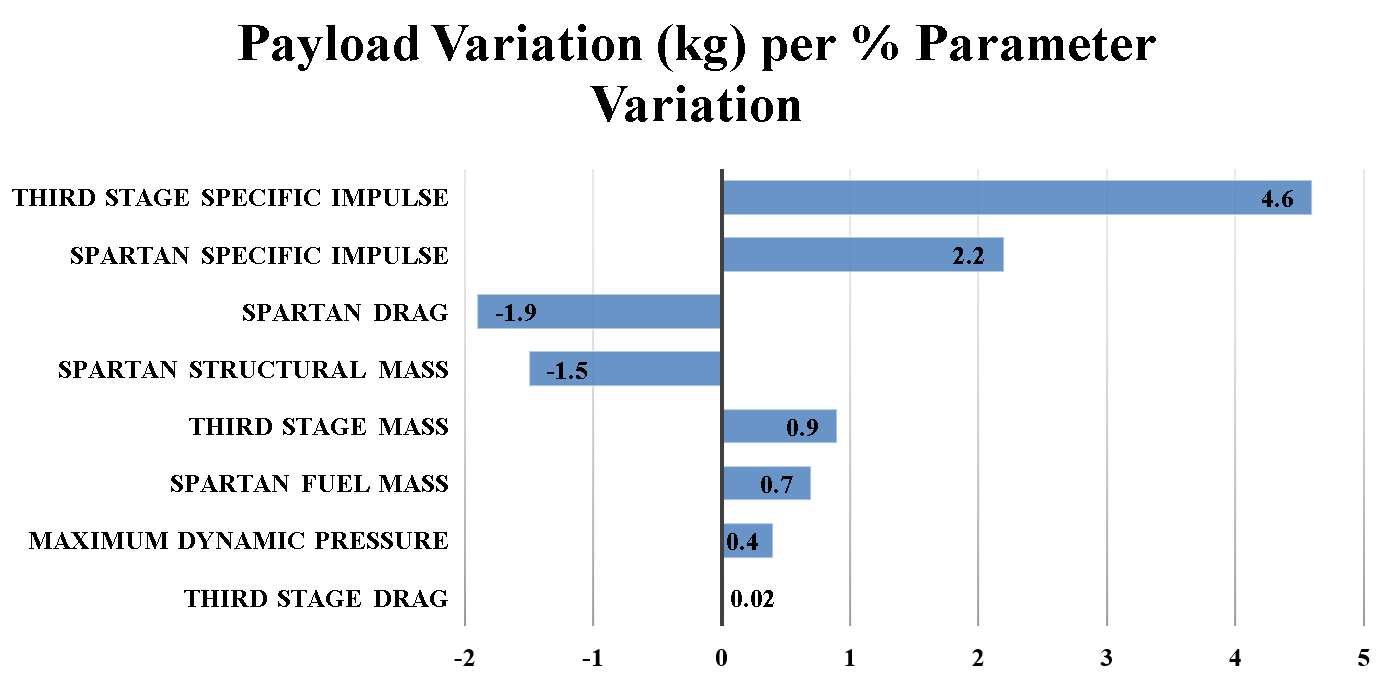
\includegraphics[width=0.99\linewidth]{figures/5_Ascent/BarChartRelativePayloadChange}
	\caption{The sensitivity of the key design parameters of the launch system.}
	\label{fig:BarChartRelativePayloadChange}
\end{figure}

The preceding sections calculate the relative sensitivity of the launch system performance to a variety of design parameters. 
Comparing and contrasting the sensitivity of the launch system to each design parameter allows for the relative impact of each design parameter to be assessed in order to inform future design decisions. 
Figure \ref{fig:BarChartRelativePayloadChange} shows the change in payload mass per percentage point variation of each design parameter. 
This change per percentage variation indicates the magnitude by which the payload-to-orbit varies as each design parameter is varied by $\pm$1\% (signs are shown for positive parameter variations, with negative signs indicating a decrease in performance), and is measure of the sensitivity of the launch system to variations in each design parameter. 
However, a 1\% variation has a significantly different implication in the context of each individual design parameter, as certain parameters can be adjusted more easily. 
As such, the change per percentage is most useful when directly assessing each design parameter, and taking into account the associated effects on other, coupled design parameters. 

The maximum dynamic pressure of the scramjet accelerator and the scramjet accelerator mass parameter are coupled directly, because the scramjet accelerator's thermal protective properties and structural strength define the maximum dynamic pressure. This means that the low variance in performance with maximum dynamic pressure may be offset by the variation in the mass of the scramjet accelerator, ie. a lower maximum dynamic pressure requires less structural and thermal protection system mass.
The relative sensitivities of the launch system to dynamic pressure (\textcolor{red}{0.9}$\frac{\Delta kg}{\Delta\%q_{max}}$), and scramjet accelerator mass ((\textcolor{red}{-1.3}$\frac{\Delta kg}{\Delta\%m_{scramjet accelerator}}$), and their absolute magnitudes (50kPa and 4957kg respectively), allow the sensitivities of these coupled effects to be directly quantified. Comparing these sensitivities implies that so long as decreasing the dynamic pressure by 1kPa allows for a reduction in structural and TPS mass of greater than \textcolor{red}{-68.6kg}, then operating the scramjet accelerator at lower dynamic pressures may be preferable. 

The influence of the fuel mass of the scramjet accelerator on the performance of the launch system is relatively low, per percentage variation. However, the fuel mass is only a fraction of the total mass of the scramjet accelerator. This means that relatively small mass changes, by kg, in fuel mass are still significant. 
When the fuel mass of the scramjet accelerator is increased, the structural mass of the tanks will require a corresponding increase. 
Comparing the impact of the fuel mass and structural mass of the scramjet accelerator along with their relative magnitudes (1562kg of fuel mass and 4957kg of structural mass), the relative impact of each is \textcolor{red}{0.7$\frac{\Delta kg_{payload}}{\Delta\%m_{scramjet accelerator fuel}}$ and -1.3$\frac{\Delta kg_{payload}}{\Delta\%m_{scramjet accelerator}}$ respectively}. This means that so long as fuel mass can be added to the scramjet accelerator with less than \textcolor{red}{1.7}kg of structural mass incorporated for each 1kg of fuel mass, adding additional fuel mass will be beneficial. However, the fuel mass is constrained considerably by th available internal space within the scramjet accelerator, which is likely to be the main limiting factor.
If the size of the fuselage of the scramjet accelerator is increased, the aerodynamic performance of the scramjet accelerator will be altered proportionally. 
The sensitivity of the launch system to the drag of the scramjet accelerator, \textcolor{red}{-2.0}$\frac{\Delta kg}{\Delta\%C_{d}}$, means that so long as 1kg of fuel can be added to the scramjet accelerator with a drag increase of less than \textcolor{red}{0.022}\%, then the maximum payload-to-orbit will increase. 


The payload-to-orbit is sensitive to the specific impulse of the C-REST engines, varying at a rate of \textcolor{red}{2.2}$\frac{\Delta kg}{\Delta\%I_{SP}}$. Increasing the specific impulse of the scramjet engines is likely to require the addition of extra systems within the scramjet engines, adding weight to the scramjet accelerator, or a change in the shape of the scramjet engines, adding drag to the scramjet accelerator. 
The slightly lower sensitivity of the launch system to the scramjet accelerator mass (\textcolor{red}{-1.3}$\frac{\Delta kg}{\Delta\%m_{scramjet accelerator}}$) compared to the sensitivity to the specific impulse, means that so long as increasing the $I_{SP}$ of the scramjet accelerator by 1\% causes a corresponding increase in the structural mass of the scramjet accelerator of less than \textcolor{red}{83.9kg}, the performance of the launch system will improve. 
The sensitivity of the launch system to variation of the scramjet accelerator drag (\textcolor{red}{-2.0}$\frac{\Delta kg}{\Delta\%C_d,{scramjet accelerator}}$) is similar in magnitude to the sensitivity to specific impulse. 
If a variation in the shape of the scramjet engines or forebody increases the $I_{SP}$ of the scramjet accelerator by 1\%, while increasing the drag of the scramjet accelerator by less than \textcolor{red}{1.1}\%, then the efficiency of the launch system will be improved. 

The aerodynamic performance (L/D) of the third stage is shown to have only a very small impact on the performance of the launch system, with a negligible drag sensitivity. This means that for any third stage shape variations, the aerodynamic sensitivity is small.
 Conversely, the specific impulse of the third stage rocket has the highest percentage payload variation effect on the launch system of any of the design parameters tested, at \textcolor{red}{11.6}$\frac{\Delta kg}{\Delta\%I_{SP,3}}$. Increasing the specific impulse of the third stage is likely to involve modifications to the engine, increasing the pressure within the fuel tanks, or adding a turbopump to assist fuel flow, all of which involve increasing the mass of the third stage rocket. 
\textcolor{red}{However, the significant nonlinearities in the response of the system to changes in the mass of the third stage mean that there is no simple relationship between these two design parameters, and that modifications to the engine of the third stage must be performed along with consideration of the entire system and its trajectory.}

 








\section{Summary}


In this chapter, LODESTAR was used to design the trajectory of the \textcolor{red}{representative} rocket-scramjet-rocket multi-stage launch system \textcolor{red}{based on the SPARTAN}. 
A trajectory was simulated in which the scramjet accelerator stage flies at a constant dynamic pressure, producing \PayloadToOrbitConstqNoReturn kg of payload-to-orbit. This trajectory served to verify LODESTAR and the simulation of  the launch system, as well as providing a baseline trajectory for comparison. 
A trajectory optimised for maximum payload-to-orbit was then calculated, which increased the payload mass to sun synchronous orbit to \PayloadToOrbitStandardNoReturn kg (an increase of \textcolor{red}{59.1}\%) compared to the constant dynamic pressure trajectory.
  The optimal flight path indicates that the optimal scramjet flight path for a system transitioning between separate airbreathing and rocket-powered stages involves the scramjet accelerator flying at less than its maximum dynamic pressure at three separate points along the trajectory. 
  Initially, the first-second stage separation occurs at a higher trajectory angle than in the constant dynamic pressure trajectory, causing the scramjet accelerator to fly at lower dynamic pressure, and trading off the exergy efficiency of the scramjet accelerator for an increase in the exergy efficiency and fuel mass of the first stage, for an overall performance gain. 
  The optimal flight path then exhibits an altitude raising manoeuvre in the middle of the trajectory, which improves the exergy efficiency of the scramjet accelerator by a very minor +0.005\%$\eta$ (+0.3\%). 
  Finally, the scramjet accelerator executes a pull-up manoeuvre before the second-third stage separation. This optimal pull-up manoeuvre trades off velocity (a decrease of \textcolor{red}{145.0}m/s) for altitude (an increase of \textcolor{red}{11.65}km) and improved flight path angle (an increase of \textcolor{red}{11.6}$^\circ$). This pull-up manoeuvre, along with the higher first-second stage separation, decreases the exergy efficiency of the scramjet accelerator by -\textcolor{red}{0.719}\%$\eta$ (-\textcolor{red}{14.04}\%) when compared to the constant dynamic pressure case. 
  However, these conditions improve the exergy efficiency of the third stage rocket significantly, by +\textcolor{red}{6.013}\%$\eta$, an increase of +\textcolor{red}{63.20}\% over the third stage released from a constant dynamic pressure trajectory. \textcolor{red}{While a pull-up manoeuvre under airbreathing operation has been identified as beneficial in previous studies\cite{Wilhite1991,Bradford2002,Fujikawa2017}, these pull-ups were either performed to lower dynamic pressure for the orbiter stage\cite{Wilhite1991,Bradford2002}, or to improve the operation of the airbreathing engines\cite{Fujikawa2017}. This study has shown that a pull-up is directly beneficial to the payload-to-orbit performance of the launch system due to the efficiency trade-offs between the stages of the launch system. This performance improvement is in addition to the possible design benefits due to heat shield and structural mass reduction of the third stage, due to the significantly lowered dynamic pressure at separation of \secondthirdSeparationqStandardNoReturn kPa, a decrease of 47.5 kPa compared to a trajectory with minimum pull-up.}


A sensitivity study was conducted, to determine the relative effects of key vehicle design parameters on the optimised trajectory. 
The maximum dynamic pressure, specific impulse, aerodynamic performance, structural mass, and fuel mass of the scramjet accelerator were modified, along with the specific impulse, mass and aerodynamic performance of the third stage, and the magnitudes of their payload-to-orbit sensitivities compared. 
The specific impulse of the third stage rocket was found to produce the most overall effect on the payload-to-orbit, increasing the payload by +\textcolor{red}{91.7}kg (+\textcolor{red}{58.6}\%) at 110\% $I_{sp}$, and decreasing the payload by -\textcolor{red}{143.9}kg (\textcolor{red}{-92.0}\%) at 95\% $I_{sp}$. However, increasing the specific impulse of the third stage rocket is likely to come at a high cost premium, which may be undesirable as the third stage is non-reusable. 
The most easily variable design factor, the maximum dynamic pressure of the scramjet accelerator, was found to have a relatively small effect on the payload-to-orbit performance of the launch system, varying the payload-to-orbit by only +\textcolor{red}{4.3}kg (+\textcolor{red}{2.7}\%) at 55kPa and -\textcolor{red}{16.1}kg (\textcolor{red}{10.3\%}) at 45kPa. The negative effect on the payload-to-orbit when flying at 45kPa is likely to be offset by the lower TPS and structural mass required by lower dynamic pressure flight. It was determined that if the TPS and structural mass decrease is greater than -\textcolor{red}{68.6}kg for every 1kPa reduction in the maximum dynamic pressure, then flying at lower dynamic pressure is potentially preferable. 







